\documentclass[a4paper,12pt]{article}
\usepackage{czech}
\usepackage[utf8]{inputenc}
\usepackage{a4wide}
\usepackage[dvipdfm]{graphicx}
\usepackage{graphics}
\usepackage{indentfirst}
\usepackage{fancyhdr}
\usepackage{setspace}
\usepackage{amsmath}
\usepackage{amssymb}
\usepackage{epsfig}

%%\usepackage{nopageno}
%%\usepackage{txfonts}
\usepackage[usenames]{color}
\renewcommand{\d}{\mbox{d}}
\newcommand{\st}{$^{\circ}$}


\begin{document}
\section{Úkol}
\begin{enumerate}
    \item Změřte V-A charakteristiky magnetronu při konstantním magnetickém poli. Rozsah napětí na magnetronu volte 0-200V (s minimálním krokem 0.1-0.3 V v oblasti skoku). Proměřte 10-15 charakteristik v rozsahu magnetizačních proudů 0-2.5i A.
    \item Pro každou naměřenou charakteristiku (při daném magnetickém poli) určete hodnotu kritického napětí (např. numerickou derivací). Získané hodnoty zpracujte graficky a určete z nich měrný náboj elektronu. Diskutujte přesnost výsledku. 
    \item Z naměřeného souboru dat vytvořte jeden graf závislosti anodového proudu magnetronem IA na magnetické indukci B při konstantním anodovém napětí UA a popište jej.
\end{enumerate}

\section{Teorie}
Magnetron je zařízení , které je principiálně elektronka s koncentrickou geometrií uvnitř magnetického pole mířícím s osou elektronky. V závislosti na velikosti magnetického pole, popř anodového napětí, poté můžeme zkoumat anodový proud. 

Měrný náboj částice je definován jako podíl náboje a hnotnosti částice. V této úloze se dá spočítat dle vzrahu
\begin{eqnarray}
\frac{e}{m_e}=\frac{8U_{A,kr}}{B^2_{kr}r_A^2}\frac{1}{\left(1-\frac{r^2_K}{r^2_A}\right)^2},
\label{w}
\end{eqnarray}
kde $U_{A,kr}$ je hodnota kritického napětí, $B_{kr}$ kritická magnetická indukce a $r$ poloměry anody a katody.

Velikost magnetické indukce pole vytvořeným dvojicí cívek v Helmotzově uspořádání je roven
\begin{eqnarray}
B=\frac{8\mu_0}{5\sqrt{5}}\frac{NI_{m}}{\rho_0}\left(1-\frac{b^2}{15\rho_0^2}\right),
\end{eqnarray}
kde $I_m$ je magnetizační proud, $\rho$ poloměr cívky, a $b$ její šířka. 


\section{Měření}
Nejprve jsem proměřil VA charakteristiky magnetronu. Nejprve jsem hrubým krokem 5 V nalezl skok. Následně jsem tento skok proměřil s krokem 0.1 V. Za pomoci programu Oracle jsem nalezl maximum derivace, které odpovídalo hodnotě kritického napětí. Charakteristiky jsem zanesl do grafů (\ref{prvni}) až (\ref{posledni}). 
Hodnoty kritických napětí jsou v tabulce \ref{TUk}.

Hondoty z tabulky \ref{TUk} jsem vynesl do grafu \ref{GUk}, kde jsem se tyto hodnoty pokusil proložit závislostí danou vztahem \ref{w}. Program gnuplot však křivku proložil, ale chyba fitu je doslova astronomická. 
Dopočtená hodnota měrného náboje
\begin{eqnarray}
\frac{e}{m_0}=173.9 \mbox{C}\cdot\mbox{kg}^{-1},
\end{eqnarray}
což se od teoretické hodnoty liší o celých 9 řádů.

Nakonec jsem z naměřených dat sestrojil graf závislosti anodového proudu magnetronem na magnetizačním rpoudu při konstantním anodovém napští, který je na obrázku \ref{GUB}. Důvod změny nezávislé proměnné je uveden v diskuzi.

\begin{table}
$$
\begin{array}{|c|c|}
\hline
I_m/\mbox{A}& U_k/\mbox{V} \\ \hline
0.5&    8.1\pm1.0 \\ \hline
0.7&    16.4\pm 1.0 \\ \hline
1.0&    33.4\pm 0.5 \\ \hline
1.1&    40.1\pm 0.7 \\ \hline
1.3&    55.6\pm 1.0 \\ \hline
1.5&    73.5\pm 0.3 \\ \hline
1.7&    93.6\pm 0.3 \\ \hline
1.9&    114.7\pm 0.3 \\ \hline
2.1&    136.5\pm 0.2 \\ \hline
\end{array}
$$
\caption{Tabulka kritických napětí}
\label{TUk}
\end{table}

\begin{figure}[h]
% GNUPLOT: LaTeX picture with Postscript
\begingroup
  \makeatletter
  \providecommand\color[2][]{%
    \GenericError{(gnuplot) \space\space\space\@spaces}{%
      Package color not loaded in conjunction with
      terminal option `colourtext'%
    }{See the gnuplot documentation for explanation.%
    }{Either use 'blacktext' in gnuplot or load the package
      color.sty in LaTeX.}%
    \renewcommand\color[2][]{}%
  }%
  \providecommand\includegraphics[2][]{%
    \GenericError{(gnuplot) \space\space\space\@spaces}{%
      Package graphicx or graphics not loaded%
    }{See the gnuplot documentation for explanation.%
    }{The gnuplot epslatex terminal needs graphicx.sty or graphics.sty.}%
    \renewcommand\includegraphics[2][]{}%
  }%
  \providecommand\rotatebox[2]{#2}%
  \@ifundefined{ifGPcolor}{%
    \newif\ifGPcolor
    \GPcolorfalse
  }{}%
  \@ifundefined{ifGPblacktext}{%
    \newif\ifGPblacktext
    \GPblacktexttrue
  }{}%
  % define a \g@addto@macro without @ in the name:
  \let\gplgaddtomacro\g@addto@macro
  % define empty templates for all commands taking text:
  \gdef\gplbacktext{}%
  \gdef\gplfronttext{}%
  \makeatother
  \ifGPblacktext
    % no textcolor at all
    \def\colorrgb#1{}%
    \def\colorgray#1{}%
  \else
    % gray or color?
    \ifGPcolor
      \def\colorrgb#1{\color[rgb]{#1}}%
      \def\colorgray#1{\color[gray]{#1}}%
      \expandafter\def\csname LTw\endcsname{\color{white}}%
      \expandafter\def\csname LTb\endcsname{\color{black}}%
      \expandafter\def\csname LTa\endcsname{\color{black}}%
      \expandafter\def\csname LT0\endcsname{\color[rgb]{1,0,0}}%
      \expandafter\def\csname LT1\endcsname{\color[rgb]{0,1,0}}%
      \expandafter\def\csname LT2\endcsname{\color[rgb]{0,0,1}}%
      \expandafter\def\csname LT3\endcsname{\color[rgb]{1,0,1}}%
      \expandafter\def\csname LT4\endcsname{\color[rgb]{0,1,1}}%
      \expandafter\def\csname LT5\endcsname{\color[rgb]{1,1,0}}%
      \expandafter\def\csname LT6\endcsname{\color[rgb]{0,0,0}}%
      \expandafter\def\csname LT7\endcsname{\color[rgb]{1,0.3,0}}%
      \expandafter\def\csname LT8\endcsname{\color[rgb]{0.5,0.5,0.5}}%
    \else
      % gray
      \def\colorrgb#1{\color{black}}%
      \def\colorgray#1{\color[gray]{#1}}%
      \expandafter\def\csname LTw\endcsname{\color{white}}%
      \expandafter\def\csname LTb\endcsname{\color{black}}%
      \expandafter\def\csname LTa\endcsname{\color{black}}%
      \expandafter\def\csname LT0\endcsname{\color{black}}%
      \expandafter\def\csname LT1\endcsname{\color{black}}%
      \expandafter\def\csname LT2\endcsname{\color{black}}%
      \expandafter\def\csname LT3\endcsname{\color{black}}%
      \expandafter\def\csname LT4\endcsname{\color{black}}%
      \expandafter\def\csname LT5\endcsname{\color{black}}%
      \expandafter\def\csname LT6\endcsname{\color{black}}%
      \expandafter\def\csname LT7\endcsname{\color{black}}%
      \expandafter\def\csname LT8\endcsname{\color{black}}%
    \fi
  \fi
  \setlength{\unitlength}{0.0500bp}%
  \begin{picture}(7200.00,5040.00)%
    \gplgaddtomacro\gplbacktext{%
      \csname LTb\endcsname%
      \put(1474,704){\makebox(0,0)[r]{\strut{} 0}}%
      \put(1474,1213){\makebox(0,0)[r]{\strut{} 0.0001}}%
      \put(1474,1722){\makebox(0,0)[r]{\strut{} 0.0002}}%
      \put(1474,2231){\makebox(0,0)[r]{\strut{} 0.0003}}%
      \put(1474,2740){\makebox(0,0)[r]{\strut{} 0.0004}}%
      \put(1474,3248){\makebox(0,0)[r]{\strut{} 0.0005}}%
      \put(1474,3757){\makebox(0,0)[r]{\strut{} 0.0006}}%
      \put(1474,4266){\makebox(0,0)[r]{\strut{} 0.0007}}%
      \put(1474,4775){\makebox(0,0)[r]{\strut{} 0.0008}}%
      \put(1606,484){\makebox(0,0){\strut{} 0}}%
      \put(2922,484){\makebox(0,0){\strut{} 50}}%
      \put(4238,484){\makebox(0,0){\strut{} 100}}%
      \put(5553,484){\makebox(0,0){\strut{} 150}}%
      \put(6869,484){\makebox(0,0){\strut{} 200}}%
      \put(308,2739){\rotatebox{-270}{\makebox(0,0){\strut{}$I_A$/A}}}%
      \put(4237,154){\makebox(0,0){\strut{}$U_A$/V}}%
    }%
    \gplgaddtomacro\gplfronttext{%
    }%
    \gplbacktext
    \put(0,0){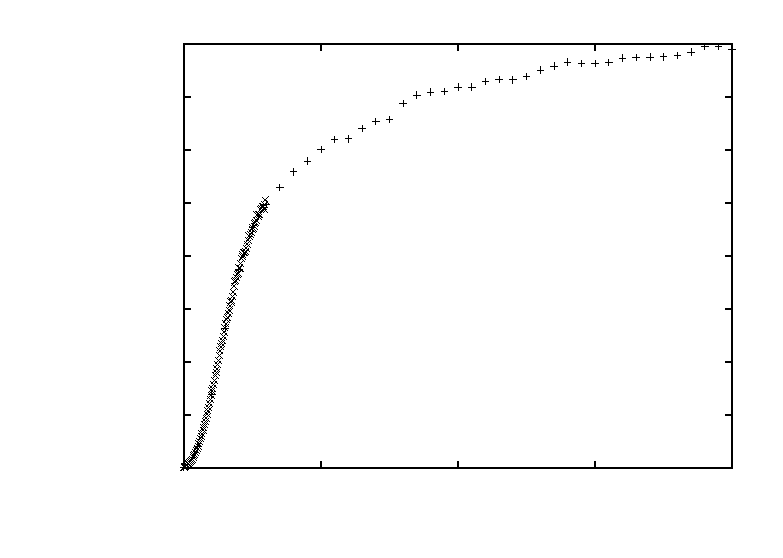
\includegraphics{0A}}%
    \gplfronttext
  \end{picture}%
\endgroup

\caption{Graf závislosti anodového proudu na napětí při magnetizačním proudu 0A.}
\label{prvni}
\end{figure}

\begin{figure}[h]
% GNUPLOT: LaTeX picture with Postscript
\begingroup
  \makeatletter
  \providecommand\color[2][]{%
    \GenericError{(gnuplot) \space\space\space\@spaces}{%
      Package color not loaded in conjunction with
      terminal option `colourtext'%
    }{See the gnuplot documentation for explanation.%
    }{Either use 'blacktext' in gnuplot or load the package
      color.sty in LaTeX.}%
    \renewcommand\color[2][]{}%
  }%
  \providecommand\includegraphics[2][]{%
    \GenericError{(gnuplot) \space\space\space\@spaces}{%
      Package graphicx or graphics not loaded%
    }{See the gnuplot documentation for explanation.%
    }{The gnuplot epslatex terminal needs graphicx.sty or graphics.sty.}%
    \renewcommand\includegraphics[2][]{}%
  }%
  \providecommand\rotatebox[2]{#2}%
  \@ifundefined{ifGPcolor}{%
    \newif\ifGPcolor
    \GPcolorfalse
  }{}%
  \@ifundefined{ifGPblacktext}{%
    \newif\ifGPblacktext
    \GPblacktexttrue
  }{}%
  % define a \g@addto@macro without @ in the name:
  \let\gplgaddtomacro\g@addto@macro
  % define empty templates for all commands taking text:
  \gdef\gplbacktext{}%
  \gdef\gplfronttext{}%
  \makeatother
  \ifGPblacktext
    % no textcolor at all
    \def\colorrgb#1{}%
    \def\colorgray#1{}%
  \else
    % gray or color?
    \ifGPcolor
      \def\colorrgb#1{\color[rgb]{#1}}%
      \def\colorgray#1{\color[gray]{#1}}%
      \expandafter\def\csname LTw\endcsname{\color{white}}%
      \expandafter\def\csname LTb\endcsname{\color{black}}%
      \expandafter\def\csname LTa\endcsname{\color{black}}%
      \expandafter\def\csname LT0\endcsname{\color[rgb]{1,0,0}}%
      \expandafter\def\csname LT1\endcsname{\color[rgb]{0,1,0}}%
      \expandafter\def\csname LT2\endcsname{\color[rgb]{0,0,1}}%
      \expandafter\def\csname LT3\endcsname{\color[rgb]{1,0,1}}%
      \expandafter\def\csname LT4\endcsname{\color[rgb]{0,1,1}}%
      \expandafter\def\csname LT5\endcsname{\color[rgb]{1,1,0}}%
      \expandafter\def\csname LT6\endcsname{\color[rgb]{0,0,0}}%
      \expandafter\def\csname LT7\endcsname{\color[rgb]{1,0.3,0}}%
      \expandafter\def\csname LT8\endcsname{\color[rgb]{0.5,0.5,0.5}}%
    \else
      % gray
      \def\colorrgb#1{\color{black}}%
      \def\colorgray#1{\color[gray]{#1}}%
      \expandafter\def\csname LTw\endcsname{\color{white}}%
      \expandafter\def\csname LTb\endcsname{\color{black}}%
      \expandafter\def\csname LTa\endcsname{\color{black}}%
      \expandafter\def\csname LT0\endcsname{\color{black}}%
      \expandafter\def\csname LT1\endcsname{\color{black}}%
      \expandafter\def\csname LT2\endcsname{\color{black}}%
      \expandafter\def\csname LT3\endcsname{\color{black}}%
      \expandafter\def\csname LT4\endcsname{\color{black}}%
      \expandafter\def\csname LT5\endcsname{\color{black}}%
      \expandafter\def\csname LT6\endcsname{\color{black}}%
      \expandafter\def\csname LT7\endcsname{\color{black}}%
      \expandafter\def\csname LT8\endcsname{\color{black}}%
    \fi
  \fi
  \setlength{\unitlength}{0.0500bp}%
  \begin{picture}(7200.00,5040.00)%
    \gplgaddtomacro\gplbacktext{%
      \csname LTb\endcsname%
      \put(1474,704){\makebox(0,0)[r]{\strut{} 0}}%
      \put(1474,1286){\makebox(0,0)[r]{\strut{} 0.0001}}%
      \put(1474,1867){\makebox(0,0)[r]{\strut{} 0.0002}}%
      \put(1474,2449){\makebox(0,0)[r]{\strut{} 0.0003}}%
      \put(1474,3030){\makebox(0,0)[r]{\strut{} 0.0004}}%
      \put(1474,3612){\makebox(0,0)[r]{\strut{} 0.0005}}%
      \put(1474,4193){\makebox(0,0)[r]{\strut{} 0.0006}}%
      \put(1474,4775){\makebox(0,0)[r]{\strut{} 0.0007}}%
      \put(1606,484){\makebox(0,0){\strut{} 0}}%
      \put(2659,484){\makebox(0,0){\strut{} 20}}%
      \put(3711,484){\makebox(0,0){\strut{} 40}}%
      \put(4764,484){\makebox(0,0){\strut{} 60}}%
      \put(5816,484){\makebox(0,0){\strut{} 80}}%
      \put(6869,484){\makebox(0,0){\strut{} 100}}%
      \put(308,2739){\rotatebox{-270}{\makebox(0,0){\strut{}$I_A$/A}}}%
      \put(4237,154){\makebox(0,0){\strut{}$U_A$/V}}%
    }%
    \gplgaddtomacro\gplfronttext{%
    }%
    \gplbacktext
    \put(0,0){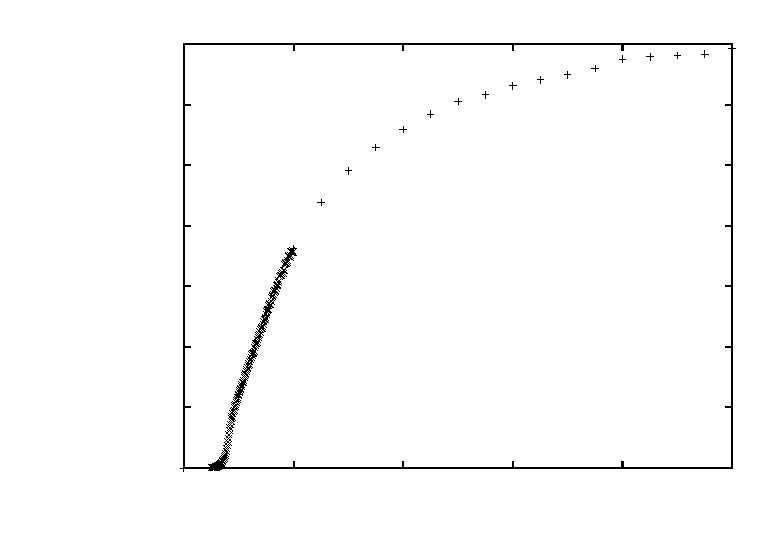
\includegraphics{0d5A}}%
    \gplfronttext
  \end{picture}%
\endgroup

\caption{Graf závislosti anodového proudu na napětí při magnetizačním proudu 0.5A.}
\end{figure}

\begin{figure}[h]
% GNUPLOT: LaTeX picture with Postscript
\begingroup
  \makeatletter
  \providecommand\color[2][]{%
    \GenericError{(gnuplot) \space\space\space\@spaces}{%
      Package color not loaded in conjunction with
      terminal option `colourtext'%
    }{See the gnuplot documentation for explanation.%
    }{Either use 'blacktext' in gnuplot or load the package
      color.sty in LaTeX.}%
    \renewcommand\color[2][]{}%
  }%
  \providecommand\includegraphics[2][]{%
    \GenericError{(gnuplot) \space\space\space\@spaces}{%
      Package graphicx or graphics not loaded%
    }{See the gnuplot documentation for explanation.%
    }{The gnuplot epslatex terminal needs graphicx.sty or graphics.sty.}%
    \renewcommand\includegraphics[2][]{}%
  }%
  \providecommand\rotatebox[2]{#2}%
  \@ifundefined{ifGPcolor}{%
    \newif\ifGPcolor
    \GPcolorfalse
  }{}%
  \@ifundefined{ifGPblacktext}{%
    \newif\ifGPblacktext
    \GPblacktexttrue
  }{}%
  % define a \g@addto@macro without @ in the name:
  \let\gplgaddtomacro\g@addto@macro
  % define empty templates for all commands taking text:
  \gdef\gplbacktext{}%
  \gdef\gplfronttext{}%
  \makeatother
  \ifGPblacktext
    % no textcolor at all
    \def\colorrgb#1{}%
    \def\colorgray#1{}%
  \else
    % gray or color?
    \ifGPcolor
      \def\colorrgb#1{\color[rgb]{#1}}%
      \def\colorgray#1{\color[gray]{#1}}%
      \expandafter\def\csname LTw\endcsname{\color{white}}%
      \expandafter\def\csname LTb\endcsname{\color{black}}%
      \expandafter\def\csname LTa\endcsname{\color{black}}%
      \expandafter\def\csname LT0\endcsname{\color[rgb]{1,0,0}}%
      \expandafter\def\csname LT1\endcsname{\color[rgb]{0,1,0}}%
      \expandafter\def\csname LT2\endcsname{\color[rgb]{0,0,1}}%
      \expandafter\def\csname LT3\endcsname{\color[rgb]{1,0,1}}%
      \expandafter\def\csname LT4\endcsname{\color[rgb]{0,1,1}}%
      \expandafter\def\csname LT5\endcsname{\color[rgb]{1,1,0}}%
      \expandafter\def\csname LT6\endcsname{\color[rgb]{0,0,0}}%
      \expandafter\def\csname LT7\endcsname{\color[rgb]{1,0.3,0}}%
      \expandafter\def\csname LT8\endcsname{\color[rgb]{0.5,0.5,0.5}}%
    \else
      % gray
      \def\colorrgb#1{\color{black}}%
      \def\colorgray#1{\color[gray]{#1}}%
      \expandafter\def\csname LTw\endcsname{\color{white}}%
      \expandafter\def\csname LTb\endcsname{\color{black}}%
      \expandafter\def\csname LTa\endcsname{\color{black}}%
      \expandafter\def\csname LT0\endcsname{\color{black}}%
      \expandafter\def\csname LT1\endcsname{\color{black}}%
      \expandafter\def\csname LT2\endcsname{\color{black}}%
      \expandafter\def\csname LT3\endcsname{\color{black}}%
      \expandafter\def\csname LT4\endcsname{\color{black}}%
      \expandafter\def\csname LT5\endcsname{\color{black}}%
      \expandafter\def\csname LT6\endcsname{\color{black}}%
      \expandafter\def\csname LT7\endcsname{\color{black}}%
      \expandafter\def\csname LT8\endcsname{\color{black}}%
    \fi
  \fi
  \setlength{\unitlength}{0.0500bp}%
  \begin{picture}(7200.00,5040.00)%
    \gplgaddtomacro\gplbacktext{%
      \csname LTb\endcsname%
      \put(1474,704){\makebox(0,0)[r]{\strut{} 0}}%
      \put(1474,1213){\makebox(0,0)[r]{\strut{} 0.0001}}%
      \put(1474,1722){\makebox(0,0)[r]{\strut{} 0.0002}}%
      \put(1474,2231){\makebox(0,0)[r]{\strut{} 0.0003}}%
      \put(1474,2740){\makebox(0,0)[r]{\strut{} 0.0004}}%
      \put(1474,3248){\makebox(0,0)[r]{\strut{} 0.0005}}%
      \put(1474,3757){\makebox(0,0)[r]{\strut{} 0.0006}}%
      \put(1474,4266){\makebox(0,0)[r]{\strut{} 0.0007}}%
      \put(1474,4775){\makebox(0,0)[r]{\strut{} 0.0008}}%
      \put(1606,484){\makebox(0,0){\strut{} 0}}%
      \put(2659,484){\makebox(0,0){\strut{} 20}}%
      \put(3711,484){\makebox(0,0){\strut{} 40}}%
      \put(4764,484){\makebox(0,0){\strut{} 60}}%
      \put(5816,484){\makebox(0,0){\strut{} 80}}%
      \put(6869,484){\makebox(0,0){\strut{} 100}}%
      \put(308,2739){\rotatebox{-270}{\makebox(0,0){\strut{}$I_A$/A}}}%
      \put(4237,154){\makebox(0,0){\strut{}$U_A$/V}}%
    }%
    \gplgaddtomacro\gplfronttext{%
    }%
    \gplbacktext
    \put(0,0){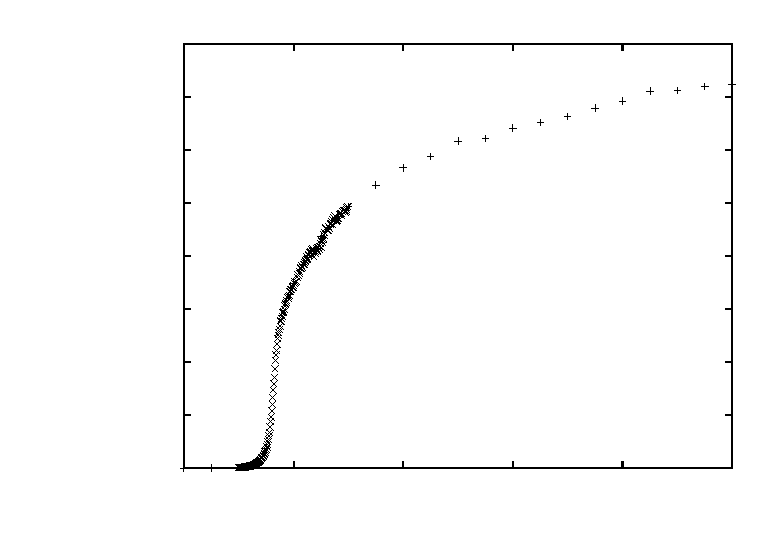
\includegraphics{0d7A}}%
    \gplfronttext
  \end{picture}%
\endgroup

\caption{Graf závislosti anodového proudu na napětí při magnetizačním proudu 0.7A.}
\end{figure}

\begin{figure}[h]
% GNUPLOT: LaTeX picture with Postscript
\begingroup
  \makeatletter
  \providecommand\color[2][]{%
    \GenericError{(gnuplot) \space\space\space\@spaces}{%
      Package color not loaded in conjunction with
      terminal option `colourtext'%
    }{See the gnuplot documentation for explanation.%
    }{Either use 'blacktext' in gnuplot or load the package
      color.sty in LaTeX.}%
    \renewcommand\color[2][]{}%
  }%
  \providecommand\includegraphics[2][]{%
    \GenericError{(gnuplot) \space\space\space\@spaces}{%
      Package graphicx or graphics not loaded%
    }{See the gnuplot documentation for explanation.%
    }{The gnuplot epslatex terminal needs graphicx.sty or graphics.sty.}%
    \renewcommand\includegraphics[2][]{}%
  }%
  \providecommand\rotatebox[2]{#2}%
  \@ifundefined{ifGPcolor}{%
    \newif\ifGPcolor
    \GPcolorfalse
  }{}%
  \@ifundefined{ifGPblacktext}{%
    \newif\ifGPblacktext
    \GPblacktexttrue
  }{}%
  % define a \g@addto@macro without @ in the name:
  \let\gplgaddtomacro\g@addto@macro
  % define empty templates for all commands taking text:
  \gdef\gplbacktext{}%
  \gdef\gplfronttext{}%
  \makeatother
  \ifGPblacktext
    % no textcolor at all
    \def\colorrgb#1{}%
    \def\colorgray#1{}%
  \else
    % gray or color?
    \ifGPcolor
      \def\colorrgb#1{\color[rgb]{#1}}%
      \def\colorgray#1{\color[gray]{#1}}%
      \expandafter\def\csname LTw\endcsname{\color{white}}%
      \expandafter\def\csname LTb\endcsname{\color{black}}%
      \expandafter\def\csname LTa\endcsname{\color{black}}%
      \expandafter\def\csname LT0\endcsname{\color[rgb]{1,0,0}}%
      \expandafter\def\csname LT1\endcsname{\color[rgb]{0,1,0}}%
      \expandafter\def\csname LT2\endcsname{\color[rgb]{0,0,1}}%
      \expandafter\def\csname LT3\endcsname{\color[rgb]{1,0,1}}%
      \expandafter\def\csname LT4\endcsname{\color[rgb]{0,1,1}}%
      \expandafter\def\csname LT5\endcsname{\color[rgb]{1,1,0}}%
      \expandafter\def\csname LT6\endcsname{\color[rgb]{0,0,0}}%
      \expandafter\def\csname LT7\endcsname{\color[rgb]{1,0.3,0}}%
      \expandafter\def\csname LT8\endcsname{\color[rgb]{0.5,0.5,0.5}}%
    \else
      % gray
      \def\colorrgb#1{\color{black}}%
      \def\colorgray#1{\color[gray]{#1}}%
      \expandafter\def\csname LTw\endcsname{\color{white}}%
      \expandafter\def\csname LTb\endcsname{\color{black}}%
      \expandafter\def\csname LTa\endcsname{\color{black}}%
      \expandafter\def\csname LT0\endcsname{\color{black}}%
      \expandafter\def\csname LT1\endcsname{\color{black}}%
      \expandafter\def\csname LT2\endcsname{\color{black}}%
      \expandafter\def\csname LT3\endcsname{\color{black}}%
      \expandafter\def\csname LT4\endcsname{\color{black}}%
      \expandafter\def\csname LT5\endcsname{\color{black}}%
      \expandafter\def\csname LT6\endcsname{\color{black}}%
      \expandafter\def\csname LT7\endcsname{\color{black}}%
      \expandafter\def\csname LT8\endcsname{\color{black}}%
    \fi
  \fi
  \setlength{\unitlength}{0.0500bp}%
  \begin{picture}(7200.00,5040.00)%
    \gplgaddtomacro\gplbacktext{%
      \csname LTb\endcsname%
      \put(1474,704){\makebox(0,0)[r]{\strut{} 0}}%
      \put(1474,1213){\makebox(0,0)[r]{\strut{} 0.0001}}%
      \put(1474,1722){\makebox(0,0)[r]{\strut{} 0.0002}}%
      \put(1474,2231){\makebox(0,0)[r]{\strut{} 0.0003}}%
      \put(1474,2740){\makebox(0,0)[r]{\strut{} 0.0004}}%
      \put(1474,3248){\makebox(0,0)[r]{\strut{} 0.0005}}%
      \put(1474,3757){\makebox(0,0)[r]{\strut{} 0.0006}}%
      \put(1474,4266){\makebox(0,0)[r]{\strut{} 0.0007}}%
      \put(1474,4775){\makebox(0,0)[r]{\strut{} 0.0008}}%
      \put(1606,484){\makebox(0,0){\strut{} 0}}%
      \put(2659,484){\makebox(0,0){\strut{} 20}}%
      \put(3711,484){\makebox(0,0){\strut{} 40}}%
      \put(4764,484){\makebox(0,0){\strut{} 60}}%
      \put(5816,484){\makebox(0,0){\strut{} 80}}%
      \put(6869,484){\makebox(0,0){\strut{} 100}}%
      \put(308,2739){\rotatebox{-270}{\makebox(0,0){\strut{}$I_A$/A}}}%
      \put(4237,154){\makebox(0,0){\strut{}$U_A$/V}}%
    }%
    \gplgaddtomacro\gplfronttext{%
    }%
    \gplbacktext
    \put(0,0){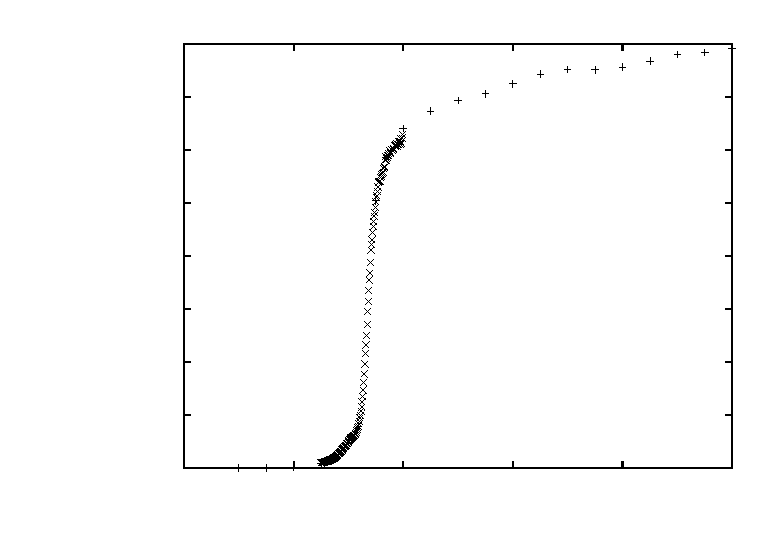
\includegraphics{1A}}%
    \gplfronttext
  \end{picture}%
\endgroup

\caption{Graf závislosti anodového proudu na napětí při magnetizačním proudu 1A.}
\end{figure}

\begin{figure}[h]
% GNUPLOT: LaTeX picture with Postscript
\begingroup
  \makeatletter
  \providecommand\color[2][]{%
    \GenericError{(gnuplot) \space\space\space\@spaces}{%
      Package color not loaded in conjunction with
      terminal option `colourtext'%
    }{See the gnuplot documentation for explanation.%
    }{Either use 'blacktext' in gnuplot or load the package
      color.sty in LaTeX.}%
    \renewcommand\color[2][]{}%
  }%
  \providecommand\includegraphics[2][]{%
    \GenericError{(gnuplot) \space\space\space\@spaces}{%
      Package graphicx or graphics not loaded%
    }{See the gnuplot documentation for explanation.%
    }{The gnuplot epslatex terminal needs graphicx.sty or graphics.sty.}%
    \renewcommand\includegraphics[2][]{}%
  }%
  \providecommand\rotatebox[2]{#2}%
  \@ifundefined{ifGPcolor}{%
    \newif\ifGPcolor
    \GPcolorfalse
  }{}%
  \@ifundefined{ifGPblacktext}{%
    \newif\ifGPblacktext
    \GPblacktexttrue
  }{}%
  % define a \g@addto@macro without @ in the name:
  \let\gplgaddtomacro\g@addto@macro
  % define empty templates for all commands taking text:
  \gdef\gplbacktext{}%
  \gdef\gplfronttext{}%
  \makeatother
  \ifGPblacktext
    % no textcolor at all
    \def\colorrgb#1{}%
    \def\colorgray#1{}%
  \else
    % gray or color?
    \ifGPcolor
      \def\colorrgb#1{\color[rgb]{#1}}%
      \def\colorgray#1{\color[gray]{#1}}%
      \expandafter\def\csname LTw\endcsname{\color{white}}%
      \expandafter\def\csname LTb\endcsname{\color{black}}%
      \expandafter\def\csname LTa\endcsname{\color{black}}%
      \expandafter\def\csname LT0\endcsname{\color[rgb]{1,0,0}}%
      \expandafter\def\csname LT1\endcsname{\color[rgb]{0,1,0}}%
      \expandafter\def\csname LT2\endcsname{\color[rgb]{0,0,1}}%
      \expandafter\def\csname LT3\endcsname{\color[rgb]{1,0,1}}%
      \expandafter\def\csname LT4\endcsname{\color[rgb]{0,1,1}}%
      \expandafter\def\csname LT5\endcsname{\color[rgb]{1,1,0}}%
      \expandafter\def\csname LT6\endcsname{\color[rgb]{0,0,0}}%
      \expandafter\def\csname LT7\endcsname{\color[rgb]{1,0.3,0}}%
      \expandafter\def\csname LT8\endcsname{\color[rgb]{0.5,0.5,0.5}}%
    \else
      % gray
      \def\colorrgb#1{\color{black}}%
      \def\colorgray#1{\color[gray]{#1}}%
      \expandafter\def\csname LTw\endcsname{\color{white}}%
      \expandafter\def\csname LTb\endcsname{\color{black}}%
      \expandafter\def\csname LTa\endcsname{\color{black}}%
      \expandafter\def\csname LT0\endcsname{\color{black}}%
      \expandafter\def\csname LT1\endcsname{\color{black}}%
      \expandafter\def\csname LT2\endcsname{\color{black}}%
      \expandafter\def\csname LT3\endcsname{\color{black}}%
      \expandafter\def\csname LT4\endcsname{\color{black}}%
      \expandafter\def\csname LT5\endcsname{\color{black}}%
      \expandafter\def\csname LT6\endcsname{\color{black}}%
      \expandafter\def\csname LT7\endcsname{\color{black}}%
      \expandafter\def\csname LT8\endcsname{\color{black}}%
    \fi
  \fi
  \setlength{\unitlength}{0.0500bp}%
  \begin{picture}(7200.00,5040.00)%
    \gplgaddtomacro\gplbacktext{%
      \csname LTb\endcsname%
      \put(1474,704){\makebox(0,0)[r]{\strut{}-0.0001}}%
      \put(1474,1156){\makebox(0,0)[r]{\strut{} 0}}%
      \put(1474,1609){\makebox(0,0)[r]{\strut{} 0.0001}}%
      \put(1474,2061){\makebox(0,0)[r]{\strut{} 0.0002}}%
      \put(1474,2513){\makebox(0,0)[r]{\strut{} 0.0003}}%
      \put(1474,2966){\makebox(0,0)[r]{\strut{} 0.0004}}%
      \put(1474,3418){\makebox(0,0)[r]{\strut{} 0.0005}}%
      \put(1474,3870){\makebox(0,0)[r]{\strut{} 0.0006}}%
      \put(1474,4323){\makebox(0,0)[r]{\strut{} 0.0007}}%
      \put(1474,4775){\makebox(0,0)[r]{\strut{} 0.0008}}%
      \put(1606,484){\makebox(0,0){\strut{} 0}}%
      \put(2659,484){\makebox(0,0){\strut{} 20}}%
      \put(3711,484){\makebox(0,0){\strut{} 40}}%
      \put(4764,484){\makebox(0,0){\strut{} 60}}%
      \put(5816,484){\makebox(0,0){\strut{} 80}}%
      \put(6869,484){\makebox(0,0){\strut{} 100}}%
      \put(308,2739){\rotatebox{-270}{\makebox(0,0){\strut{}$I_A$/A}}}%
      \put(4237,154){\makebox(0,0){\strut{}$U_A$/V}}%
    }%
    \gplgaddtomacro\gplfronttext{%
    }%
    \gplbacktext
    \put(0,0){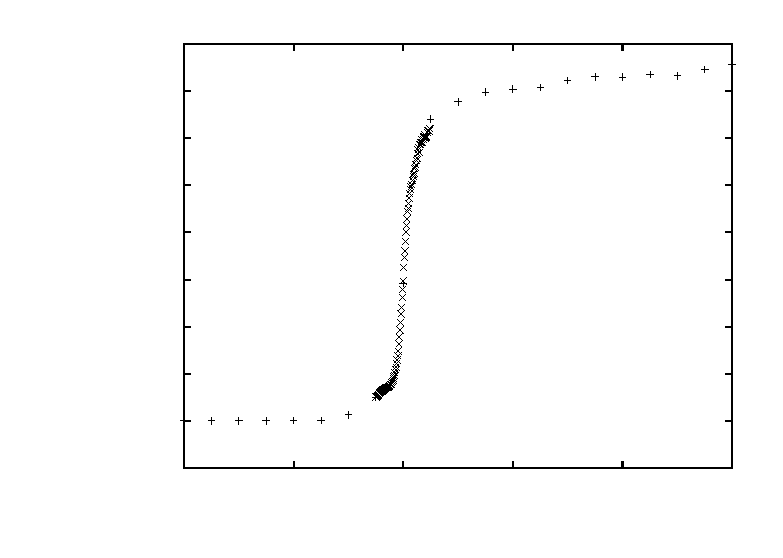
\includegraphics{1d1A}}%
    \gplfronttext
  \end{picture}%
\endgroup

\caption{Graf závislosti anodového proudu na napětí při magnetizačním proudu 1.1A.}
\end{figure}

\begin{figure}[h]
% GNUPLOT: LaTeX picture with Postscript
\begingroup
  \makeatletter
  \providecommand\color[2][]{%
    \GenericError{(gnuplot) \space\space\space\@spaces}{%
      Package color not loaded in conjunction with
      terminal option `colourtext'%
    }{See the gnuplot documentation for explanation.%
    }{Either use 'blacktext' in gnuplot or load the package
      color.sty in LaTeX.}%
    \renewcommand\color[2][]{}%
  }%
  \providecommand\includegraphics[2][]{%
    \GenericError{(gnuplot) \space\space\space\@spaces}{%
      Package graphicx or graphics not loaded%
    }{See the gnuplot documentation for explanation.%
    }{The gnuplot epslatex terminal needs graphicx.sty or graphics.sty.}%
    \renewcommand\includegraphics[2][]{}%
  }%
  \providecommand\rotatebox[2]{#2}%
  \@ifundefined{ifGPcolor}{%
    \newif\ifGPcolor
    \GPcolorfalse
  }{}%
  \@ifundefined{ifGPblacktext}{%
    \newif\ifGPblacktext
    \GPblacktexttrue
  }{}%
  % define a \g@addto@macro without @ in the name:
  \let\gplgaddtomacro\g@addto@macro
  % define empty templates for all commands taking text:
  \gdef\gplbacktext{}%
  \gdef\gplfronttext{}%
  \makeatother
  \ifGPblacktext
    % no textcolor at all
    \def\colorrgb#1{}%
    \def\colorgray#1{}%
  \else
    % gray or color?
    \ifGPcolor
      \def\colorrgb#1{\color[rgb]{#1}}%
      \def\colorgray#1{\color[gray]{#1}}%
      \expandafter\def\csname LTw\endcsname{\color{white}}%
      \expandafter\def\csname LTb\endcsname{\color{black}}%
      \expandafter\def\csname LTa\endcsname{\color{black}}%
      \expandafter\def\csname LT0\endcsname{\color[rgb]{1,0,0}}%
      \expandafter\def\csname LT1\endcsname{\color[rgb]{0,1,0}}%
      \expandafter\def\csname LT2\endcsname{\color[rgb]{0,0,1}}%
      \expandafter\def\csname LT3\endcsname{\color[rgb]{1,0,1}}%
      \expandafter\def\csname LT4\endcsname{\color[rgb]{0,1,1}}%
      \expandafter\def\csname LT5\endcsname{\color[rgb]{1,1,0}}%
      \expandafter\def\csname LT6\endcsname{\color[rgb]{0,0,0}}%
      \expandafter\def\csname LT7\endcsname{\color[rgb]{1,0.3,0}}%
      \expandafter\def\csname LT8\endcsname{\color[rgb]{0.5,0.5,0.5}}%
    \else
      % gray
      \def\colorrgb#1{\color{black}}%
      \def\colorgray#1{\color[gray]{#1}}%
      \expandafter\def\csname LTw\endcsname{\color{white}}%
      \expandafter\def\csname LTb\endcsname{\color{black}}%
      \expandafter\def\csname LTa\endcsname{\color{black}}%
      \expandafter\def\csname LT0\endcsname{\color{black}}%
      \expandafter\def\csname LT1\endcsname{\color{black}}%
      \expandafter\def\csname LT2\endcsname{\color{black}}%
      \expandafter\def\csname LT3\endcsname{\color{black}}%
      \expandafter\def\csname LT4\endcsname{\color{black}}%
      \expandafter\def\csname LT5\endcsname{\color{black}}%
      \expandafter\def\csname LT6\endcsname{\color{black}}%
      \expandafter\def\csname LT7\endcsname{\color{black}}%
      \expandafter\def\csname LT8\endcsname{\color{black}}%
    \fi
  \fi
  \setlength{\unitlength}{0.0500bp}%
  \begin{picture}(7200.00,5040.00)%
    \gplgaddtomacro\gplbacktext{%
      \csname LTb\endcsname%
      \put(1474,704){\makebox(0,0)[r]{\strut{} 0}}%
      \put(1474,1213){\makebox(0,0)[r]{\strut{} 0.0001}}%
      \put(1474,1722){\makebox(0,0)[r]{\strut{} 0.0002}}%
      \put(1474,2231){\makebox(0,0)[r]{\strut{} 0.0003}}%
      \put(1474,2740){\makebox(0,0)[r]{\strut{} 0.0004}}%
      \put(1474,3248){\makebox(0,0)[r]{\strut{} 0.0005}}%
      \put(1474,3757){\makebox(0,0)[r]{\strut{} 0.0006}}%
      \put(1474,4266){\makebox(0,0)[r]{\strut{} 0.0007}}%
      \put(1474,4775){\makebox(0,0)[r]{\strut{} 0.0008}}%
      \put(1606,484){\makebox(0,0){\strut{} 0}}%
      \put(2659,484){\makebox(0,0){\strut{} 20}}%
      \put(3711,484){\makebox(0,0){\strut{} 40}}%
      \put(4764,484){\makebox(0,0){\strut{} 60}}%
      \put(5816,484){\makebox(0,0){\strut{} 80}}%
      \put(6869,484){\makebox(0,0){\strut{} 100}}%
      \put(308,2739){\rotatebox{-270}{\makebox(0,0){\strut{}$I_A$/A}}}%
      \put(4237,154){\makebox(0,0){\strut{}$U_A$/V}}%
    }%
    \gplgaddtomacro\gplfronttext{%
    }%
    \gplbacktext
    \put(0,0){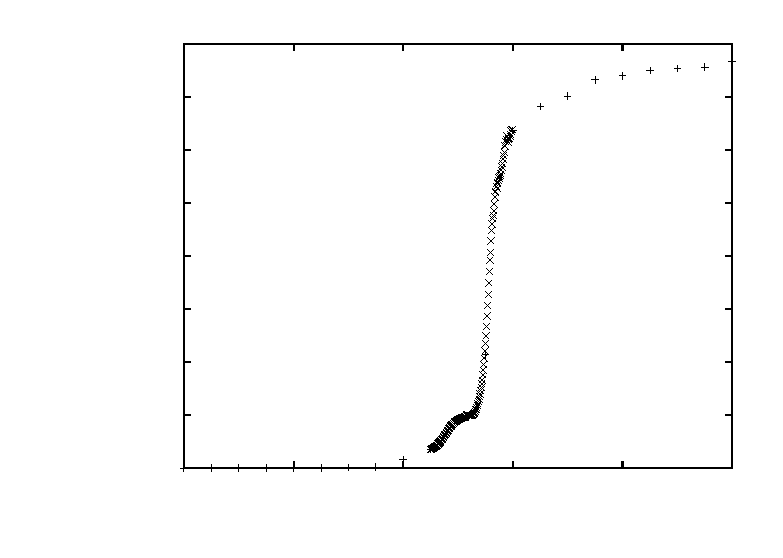
\includegraphics{1d3A}}%
    \gplfronttext
  \end{picture}%
\endgroup

\caption{Graf závislosti anodového proudu na napětí při magnetizačním proudu 1.3A.}  
\end{figure}


\begin{figure}[h]
% GNUPLOT: LaTeX picture with Postscript
\begingroup
  \makeatletter
  \providecommand\color[2][]{%
    \GenericError{(gnuplot) \space\space\space\@spaces}{%
      Package color not loaded in conjunction with
      terminal option `colourtext'%
    }{See the gnuplot documentation for explanation.%
    }{Either use 'blacktext' in gnuplot or load the package
      color.sty in LaTeX.}%
    \renewcommand\color[2][]{}%
  }%
  \providecommand\includegraphics[2][]{%
    \GenericError{(gnuplot) \space\space\space\@spaces}{%
      Package graphicx or graphics not loaded%
    }{See the gnuplot documentation for explanation.%
    }{The gnuplot epslatex terminal needs graphicx.sty or graphics.sty.}%
    \renewcommand\includegraphics[2][]{}%
  }%
  \providecommand\rotatebox[2]{#2}%
  \@ifundefined{ifGPcolor}{%
    \newif\ifGPcolor
    \GPcolorfalse
  }{}%
  \@ifundefined{ifGPblacktext}{%
    \newif\ifGPblacktext
    \GPblacktexttrue
  }{}%
  % define a \g@addto@macro without @ in the name:
  \let\gplgaddtomacro\g@addto@macro
  % define empty templates for all commands taking text:
  \gdef\gplbacktext{}%
  \gdef\gplfronttext{}%
  \makeatother
  \ifGPblacktext
    % no textcolor at all
    \def\colorrgb#1{}%
    \def\colorgray#1{}%
  \else
    % gray or color?
    \ifGPcolor
      \def\colorrgb#1{\color[rgb]{#1}}%
      \def\colorgray#1{\color[gray]{#1}}%
      \expandafter\def\csname LTw\endcsname{\color{white}}%
      \expandafter\def\csname LTb\endcsname{\color{black}}%
      \expandafter\def\csname LTa\endcsname{\color{black}}%
      \expandafter\def\csname LT0\endcsname{\color[rgb]{1,0,0}}%
      \expandafter\def\csname LT1\endcsname{\color[rgb]{0,1,0}}%
      \expandafter\def\csname LT2\endcsname{\color[rgb]{0,0,1}}%
      \expandafter\def\csname LT3\endcsname{\color[rgb]{1,0,1}}%
      \expandafter\def\csname LT4\endcsname{\color[rgb]{0,1,1}}%
      \expandafter\def\csname LT5\endcsname{\color[rgb]{1,1,0}}%
      \expandafter\def\csname LT6\endcsname{\color[rgb]{0,0,0}}%
      \expandafter\def\csname LT7\endcsname{\color[rgb]{1,0.3,0}}%
      \expandafter\def\csname LT8\endcsname{\color[rgb]{0.5,0.5,0.5}}%
    \else
      % gray
      \def\colorrgb#1{\color{black}}%
      \def\colorgray#1{\color[gray]{#1}}%
      \expandafter\def\csname LTw\endcsname{\color{white}}%
      \expandafter\def\csname LTb\endcsname{\color{black}}%
      \expandafter\def\csname LTa\endcsname{\color{black}}%
      \expandafter\def\csname LT0\endcsname{\color{black}}%
      \expandafter\def\csname LT1\endcsname{\color{black}}%
      \expandafter\def\csname LT2\endcsname{\color{black}}%
      \expandafter\def\csname LT3\endcsname{\color{black}}%
      \expandafter\def\csname LT4\endcsname{\color{black}}%
      \expandafter\def\csname LT5\endcsname{\color{black}}%
      \expandafter\def\csname LT6\endcsname{\color{black}}%
      \expandafter\def\csname LT7\endcsname{\color{black}}%
      \expandafter\def\csname LT8\endcsname{\color{black}}%
    \fi
  \fi
  \setlength{\unitlength}{0.0500bp}%
  \begin{picture}(7200.00,5040.00)%
    \gplgaddtomacro\gplbacktext{%
      \csname LTb\endcsname%
      \put(1474,704){\makebox(0,0)[r]{\strut{} 0}}%
      \put(1474,1213){\makebox(0,0)[r]{\strut{} 0.0001}}%
      \put(1474,1722){\makebox(0,0)[r]{\strut{} 0.0002}}%
      \put(1474,2231){\makebox(0,0)[r]{\strut{} 0.0003}}%
      \put(1474,2740){\makebox(0,0)[r]{\strut{} 0.0004}}%
      \put(1474,3248){\makebox(0,0)[r]{\strut{} 0.0005}}%
      \put(1474,3757){\makebox(0,0)[r]{\strut{} 0.0006}}%
      \put(1474,4266){\makebox(0,0)[r]{\strut{} 0.0007}}%
      \put(1474,4775){\makebox(0,0)[r]{\strut{} 0.0008}}%
      \put(1606,484){\makebox(0,0){\strut{} 0}}%
      \put(2659,484){\makebox(0,0){\strut{} 20}}%
      \put(3711,484){\makebox(0,0){\strut{} 40}}%
      \put(4764,484){\makebox(0,0){\strut{} 60}}%
      \put(5816,484){\makebox(0,0){\strut{} 80}}%
      \put(6869,484){\makebox(0,0){\strut{} 100}}%
      \put(308,2739){\rotatebox{-270}{\makebox(0,0){\strut{}$I_A$/A}}}%
      \put(4237,154){\makebox(0,0){\strut{}$U_A$/V}}%
    }%
    \gplgaddtomacro\gplfronttext{%
    }%
    \gplbacktext
    \put(0,0){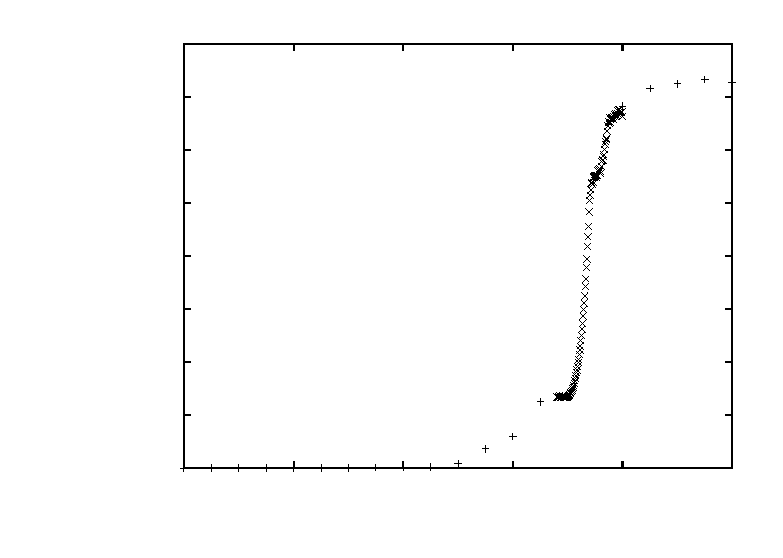
\includegraphics{1d5A}}%
    \gplfronttext
  \end{picture}%
\endgroup

\caption{Graf závislosti anodového proudu na napětí při magnetizačním proudu 1.5A.}
\end{figure}

\begin{figure}[h]
% GNUPLOT: LaTeX picture with Postscript
\begingroup
  \makeatletter
  \providecommand\color[2][]{%
    \GenericError{(gnuplot) \space\space\space\@spaces}{%
      Package color not loaded in conjunction with
      terminal option `colourtext'%
    }{See the gnuplot documentation for explanation.%
    }{Either use 'blacktext' in gnuplot or load the package
      color.sty in LaTeX.}%
    \renewcommand\color[2][]{}%
  }%
  \providecommand\includegraphics[2][]{%
    \GenericError{(gnuplot) \space\space\space\@spaces}{%
      Package graphicx or graphics not loaded%
    }{See the gnuplot documentation for explanation.%
    }{The gnuplot epslatex terminal needs graphicx.sty or graphics.sty.}%
    \renewcommand\includegraphics[2][]{}%
  }%
  \providecommand\rotatebox[2]{#2}%
  \@ifundefined{ifGPcolor}{%
    \newif\ifGPcolor
    \GPcolorfalse
  }{}%
  \@ifundefined{ifGPblacktext}{%
    \newif\ifGPblacktext
    \GPblacktexttrue
  }{}%
  % define a \g@addto@macro without @ in the name:
  \let\gplgaddtomacro\g@addto@macro
  % define empty templates for all commands taking text:
  \gdef\gplbacktext{}%
  \gdef\gplfronttext{}%
  \makeatother
  \ifGPblacktext
    % no textcolor at all
    \def\colorrgb#1{}%
    \def\colorgray#1{}%
  \else
    % gray or color?
    \ifGPcolor
      \def\colorrgb#1{\color[rgb]{#1}}%
      \def\colorgray#1{\color[gray]{#1}}%
      \expandafter\def\csname LTw\endcsname{\color{white}}%
      \expandafter\def\csname LTb\endcsname{\color{black}}%
      \expandafter\def\csname LTa\endcsname{\color{black}}%
      \expandafter\def\csname LT0\endcsname{\color[rgb]{1,0,0}}%
      \expandafter\def\csname LT1\endcsname{\color[rgb]{0,1,0}}%
      \expandafter\def\csname LT2\endcsname{\color[rgb]{0,0,1}}%
      \expandafter\def\csname LT3\endcsname{\color[rgb]{1,0,1}}%
      \expandafter\def\csname LT4\endcsname{\color[rgb]{0,1,1}}%
      \expandafter\def\csname LT5\endcsname{\color[rgb]{1,1,0}}%
      \expandafter\def\csname LT6\endcsname{\color[rgb]{0,0,0}}%
      \expandafter\def\csname LT7\endcsname{\color[rgb]{1,0.3,0}}%
      \expandafter\def\csname LT8\endcsname{\color[rgb]{0.5,0.5,0.5}}%
    \else
      % gray
      \def\colorrgb#1{\color{black}}%
      \def\colorgray#1{\color[gray]{#1}}%
      \expandafter\def\csname LTw\endcsname{\color{white}}%
      \expandafter\def\csname LTb\endcsname{\color{black}}%
      \expandafter\def\csname LTa\endcsname{\color{black}}%
      \expandafter\def\csname LT0\endcsname{\color{black}}%
      \expandafter\def\csname LT1\endcsname{\color{black}}%
      \expandafter\def\csname LT2\endcsname{\color{black}}%
      \expandafter\def\csname LT3\endcsname{\color{black}}%
      \expandafter\def\csname LT4\endcsname{\color{black}}%
      \expandafter\def\csname LT5\endcsname{\color{black}}%
      \expandafter\def\csname LT6\endcsname{\color{black}}%
      \expandafter\def\csname LT7\endcsname{\color{black}}%
      \expandafter\def\csname LT8\endcsname{\color{black}}%
    \fi
  \fi
  \setlength{\unitlength}{0.0500bp}%
  \begin{picture}(7200.00,5040.00)%
    \gplgaddtomacro\gplbacktext{%
      \csname LTb\endcsname%
      \put(1474,704){\makebox(0,0)[r]{\strut{} 0}}%
      \put(1474,1213){\makebox(0,0)[r]{\strut{} 0.0001}}%
      \put(1474,1722){\makebox(0,0)[r]{\strut{} 0.0002}}%
      \put(1474,2231){\makebox(0,0)[r]{\strut{} 0.0003}}%
      \put(1474,2740){\makebox(0,0)[r]{\strut{} 0.0004}}%
      \put(1474,3248){\makebox(0,0)[r]{\strut{} 0.0005}}%
      \put(1474,3757){\makebox(0,0)[r]{\strut{} 0.0006}}%
      \put(1474,4266){\makebox(0,0)[r]{\strut{} 0.0007}}%
      \put(1474,4775){\makebox(0,0)[r]{\strut{} 0.0008}}%
      \put(1606,484){\makebox(0,0){\strut{} 0}}%
      \put(2264,484){\makebox(0,0){\strut{} 20}}%
      \put(2922,484){\makebox(0,0){\strut{} 40}}%
      \put(3580,484){\makebox(0,0){\strut{} 60}}%
      \put(4237,484){\makebox(0,0){\strut{} 80}}%
      \put(4895,484){\makebox(0,0){\strut{} 100}}%
      \put(5553,484){\makebox(0,0){\strut{} 120}}%
      \put(6211,484){\makebox(0,0){\strut{} 140}}%
      \put(6869,484){\makebox(0,0){\strut{} 160}}%
      \put(308,2739){\rotatebox{-270}{\makebox(0,0){\strut{}$I_A$/A}}}%
      \put(4237,154){\makebox(0,0){\strut{}$U_A$/V}}%
    }%
    \gplgaddtomacro\gplfronttext{%
    }%
    \gplbacktext
    \put(0,0){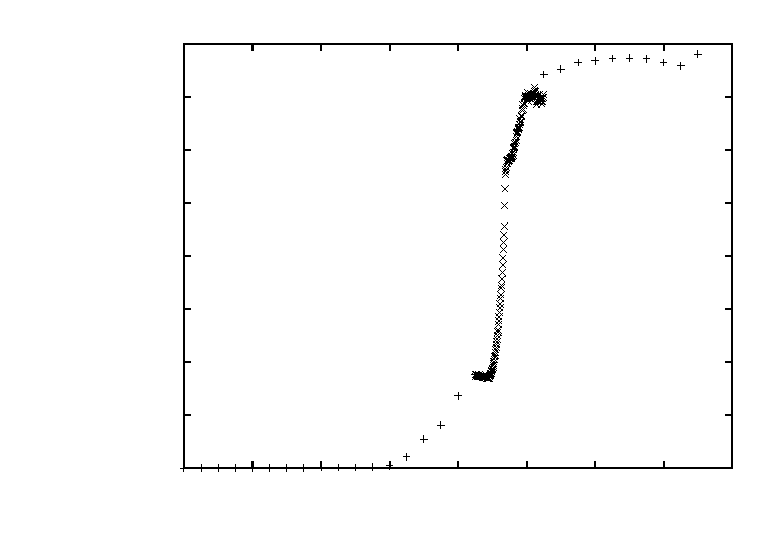
\includegraphics{1d7A}}%
    \gplfronttext
  \end{picture}%
\endgroup

\caption{Graf závislosti anodového proudu na napětí při magnetizačním proudu 1.7A.}
\end{figure}

\begin{figure}[h]
% GNUPLOT: LaTeX picture with Postscript
\begingroup
  \makeatletter
  \providecommand\color[2][]{%
    \GenericError{(gnuplot) \space\space\space\@spaces}{%
      Package color not loaded in conjunction with
      terminal option `colourtext'%
    }{See the gnuplot documentation for explanation.%
    }{Either use 'blacktext' in gnuplot or load the package
      color.sty in LaTeX.}%
    \renewcommand\color[2][]{}%
  }%
  \providecommand\includegraphics[2][]{%
    \GenericError{(gnuplot) \space\space\space\@spaces}{%
      Package graphicx or graphics not loaded%
    }{See the gnuplot documentation for explanation.%
    }{The gnuplot epslatex terminal needs graphicx.sty or graphics.sty.}%
    \renewcommand\includegraphics[2][]{}%
  }%
  \providecommand\rotatebox[2]{#2}%
  \@ifundefined{ifGPcolor}{%
    \newif\ifGPcolor
    \GPcolorfalse
  }{}%
  \@ifundefined{ifGPblacktext}{%
    \newif\ifGPblacktext
    \GPblacktexttrue
  }{}%
  % define a \g@addto@macro without @ in the name:
  \let\gplgaddtomacro\g@addto@macro
  % define empty templates for all commands taking text:
  \gdef\gplbacktext{}%
  \gdef\gplfronttext{}%
  \makeatother
  \ifGPblacktext
    % no textcolor at all
    \def\colorrgb#1{}%
    \def\colorgray#1{}%
  \else
    % gray or color?
    \ifGPcolor
      \def\colorrgb#1{\color[rgb]{#1}}%
      \def\colorgray#1{\color[gray]{#1}}%
      \expandafter\def\csname LTw\endcsname{\color{white}}%
      \expandafter\def\csname LTb\endcsname{\color{black}}%
      \expandafter\def\csname LTa\endcsname{\color{black}}%
      \expandafter\def\csname LT0\endcsname{\color[rgb]{1,0,0}}%
      \expandafter\def\csname LT1\endcsname{\color[rgb]{0,1,0}}%
      \expandafter\def\csname LT2\endcsname{\color[rgb]{0,0,1}}%
      \expandafter\def\csname LT3\endcsname{\color[rgb]{1,0,1}}%
      \expandafter\def\csname LT4\endcsname{\color[rgb]{0,1,1}}%
      \expandafter\def\csname LT5\endcsname{\color[rgb]{1,1,0}}%
      \expandafter\def\csname LT6\endcsname{\color[rgb]{0,0,0}}%
      \expandafter\def\csname LT7\endcsname{\color[rgb]{1,0.3,0}}%
      \expandafter\def\csname LT8\endcsname{\color[rgb]{0.5,0.5,0.5}}%
    \else
      % gray
      \def\colorrgb#1{\color{black}}%
      \def\colorgray#1{\color[gray]{#1}}%
      \expandafter\def\csname LTw\endcsname{\color{white}}%
      \expandafter\def\csname LTb\endcsname{\color{black}}%
      \expandafter\def\csname LTa\endcsname{\color{black}}%
      \expandafter\def\csname LT0\endcsname{\color{black}}%
      \expandafter\def\csname LT1\endcsname{\color{black}}%
      \expandafter\def\csname LT2\endcsname{\color{black}}%
      \expandafter\def\csname LT3\endcsname{\color{black}}%
      \expandafter\def\csname LT4\endcsname{\color{black}}%
      \expandafter\def\csname LT5\endcsname{\color{black}}%
      \expandafter\def\csname LT6\endcsname{\color{black}}%
      \expandafter\def\csname LT7\endcsname{\color{black}}%
      \expandafter\def\csname LT8\endcsname{\color{black}}%
    \fi
  \fi
  \setlength{\unitlength}{0.0500bp}%
  \begin{picture}(7200.00,5040.00)%
    \gplgaddtomacro\gplbacktext{%
      \csname LTb\endcsname%
      \put(1474,704){\makebox(0,0)[r]{\strut{} 0}}%
      \put(1474,1213){\makebox(0,0)[r]{\strut{} 0.0001}}%
      \put(1474,1722){\makebox(0,0)[r]{\strut{} 0.0002}}%
      \put(1474,2231){\makebox(0,0)[r]{\strut{} 0.0003}}%
      \put(1474,2740){\makebox(0,0)[r]{\strut{} 0.0004}}%
      \put(1474,3248){\makebox(0,0)[r]{\strut{} 0.0005}}%
      \put(1474,3757){\makebox(0,0)[r]{\strut{} 0.0006}}%
      \put(1474,4266){\makebox(0,0)[r]{\strut{} 0.0007}}%
      \put(1474,4775){\makebox(0,0)[r]{\strut{} 0.0008}}%
      \put(1606,484){\makebox(0,0){\strut{} 40}}%
      \put(2483,484){\makebox(0,0){\strut{} 60}}%
      \put(3360,484){\makebox(0,0){\strut{} 80}}%
      \put(4238,484){\makebox(0,0){\strut{} 100}}%
      \put(5115,484){\makebox(0,0){\strut{} 120}}%
      \put(5992,484){\makebox(0,0){\strut{} 140}}%
      \put(6869,484){\makebox(0,0){\strut{} 160}}%
      \put(308,2739){\rotatebox{-270}{\makebox(0,0){\strut{}$I_A$/A}}}%
      \put(4237,154){\makebox(0,0){\strut{}$U_A$/V}}%
    }%
    \gplgaddtomacro\gplfronttext{%
    }%
    \gplbacktext
    \put(0,0){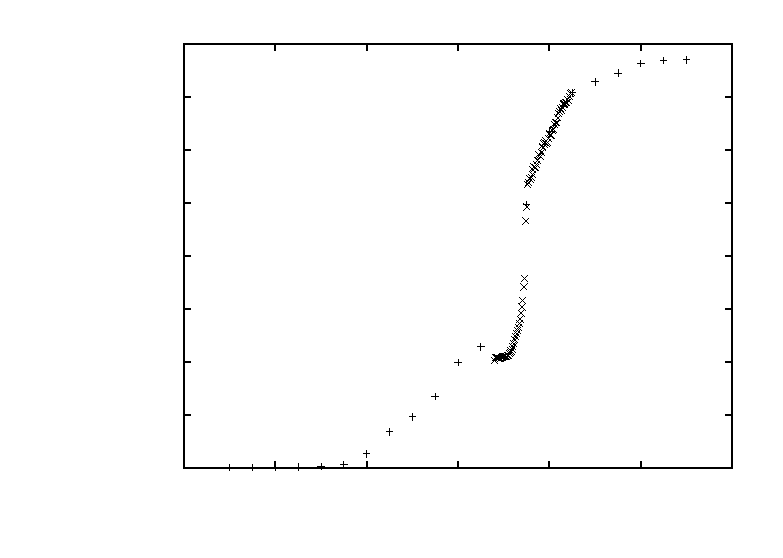
\includegraphics{1d9A}}%
    \gplfronttext
  \end{picture}%
\endgroup

\caption{Graf závislosti anodového proudu na napětí při magnetizačním proudu 1.9A.}
\end{figure}

\begin{figure}[h]
% GNUPLOT: LaTeX picture with Postscript
\begingroup
  \makeatletter
  \providecommand\color[2][]{%
    \GenericError{(gnuplot) \space\space\space\@spaces}{%
      Package color not loaded in conjunction with
      terminal option `colourtext'%
    }{See the gnuplot documentation for explanation.%
    }{Either use 'blacktext' in gnuplot or load the package
      color.sty in LaTeX.}%
    \renewcommand\color[2][]{}%
  }%
  \providecommand\includegraphics[2][]{%
    \GenericError{(gnuplot) \space\space\space\@spaces}{%
      Package graphicx or graphics not loaded%
    }{See the gnuplot documentation for explanation.%
    }{The gnuplot epslatex terminal needs graphicx.sty or graphics.sty.}%
    \renewcommand\includegraphics[2][]{}%
  }%
  \providecommand\rotatebox[2]{#2}%
  \@ifundefined{ifGPcolor}{%
    \newif\ifGPcolor
    \GPcolorfalse
  }{}%
  \@ifundefined{ifGPblacktext}{%
    \newif\ifGPblacktext
    \GPblacktexttrue
  }{}%
  % define a \g@addto@macro without @ in the name:
  \let\gplgaddtomacro\g@addto@macro
  % define empty templates for all commands taking text:
  \gdef\gplbacktext{}%
  \gdef\gplfronttext{}%
  \makeatother
  \ifGPblacktext
    % no textcolor at all
    \def\colorrgb#1{}%
    \def\colorgray#1{}%
  \else
    % gray or color?
    \ifGPcolor
      \def\colorrgb#1{\color[rgb]{#1}}%
      \def\colorgray#1{\color[gray]{#1}}%
      \expandafter\def\csname LTw\endcsname{\color{white}}%
      \expandafter\def\csname LTb\endcsname{\color{black}}%
      \expandafter\def\csname LTa\endcsname{\color{black}}%
      \expandafter\def\csname LT0\endcsname{\color[rgb]{1,0,0}}%
      \expandafter\def\csname LT1\endcsname{\color[rgb]{0,1,0}}%
      \expandafter\def\csname LT2\endcsname{\color[rgb]{0,0,1}}%
      \expandafter\def\csname LT3\endcsname{\color[rgb]{1,0,1}}%
      \expandafter\def\csname LT4\endcsname{\color[rgb]{0,1,1}}%
      \expandafter\def\csname LT5\endcsname{\color[rgb]{1,1,0}}%
      \expandafter\def\csname LT6\endcsname{\color[rgb]{0,0,0}}%
      \expandafter\def\csname LT7\endcsname{\color[rgb]{1,0.3,0}}%
      \expandafter\def\csname LT8\endcsname{\color[rgb]{0.5,0.5,0.5}}%
    \else
      % gray
      \def\colorrgb#1{\color{black}}%
      \def\colorgray#1{\color[gray]{#1}}%
      \expandafter\def\csname LTw\endcsname{\color{white}}%
      \expandafter\def\csname LTb\endcsname{\color{black}}%
      \expandafter\def\csname LTa\endcsname{\color{black}}%
      \expandafter\def\csname LT0\endcsname{\color{black}}%
      \expandafter\def\csname LT1\endcsname{\color{black}}%
      \expandafter\def\csname LT2\endcsname{\color{black}}%
      \expandafter\def\csname LT3\endcsname{\color{black}}%
      \expandafter\def\csname LT4\endcsname{\color{black}}%
      \expandafter\def\csname LT5\endcsname{\color{black}}%
      \expandafter\def\csname LT6\endcsname{\color{black}}%
      \expandafter\def\csname LT7\endcsname{\color{black}}%
      \expandafter\def\csname LT8\endcsname{\color{black}}%
    \fi
  \fi
  \setlength{\unitlength}{0.0500bp}%
  \begin{picture}(7200.00,5040.00)%
    \gplgaddtomacro\gplbacktext{%
      \csname LTb\endcsname%
      \put(1474,704){\makebox(0,0)[r]{\strut{} 0}}%
      \put(1474,1213){\makebox(0,0)[r]{\strut{} 0.0001}}%
      \put(1474,1722){\makebox(0,0)[r]{\strut{} 0.0002}}%
      \put(1474,2231){\makebox(0,0)[r]{\strut{} 0.0003}}%
      \put(1474,2740){\makebox(0,0)[r]{\strut{} 0.0004}}%
      \put(1474,3248){\makebox(0,0)[r]{\strut{} 0.0005}}%
      \put(1474,3757){\makebox(0,0)[r]{\strut{} 0.0006}}%
      \put(1474,4266){\makebox(0,0)[r]{\strut{} 0.0007}}%
      \put(1474,4775){\makebox(0,0)[r]{\strut{} 0.0008}}%
      \put(1606,484){\makebox(0,0){\strut{} 80}}%
      \put(2659,484){\makebox(0,0){\strut{} 100}}%
      \put(3711,484){\makebox(0,0){\strut{} 120}}%
      \put(4764,484){\makebox(0,0){\strut{} 140}}%
      \put(5816,484){\makebox(0,0){\strut{} 160}}%
      \put(6869,484){\makebox(0,0){\strut{} 180}}%
      \put(308,2739){\rotatebox{-270}{\makebox(0,0){\strut{}$I_A$/A}}}%
      \put(4237,154){\makebox(0,0){\strut{}$U_A$/V}}%
    }%
    \gplgaddtomacro\gplfronttext{%
    }%
    \gplbacktext
    \put(0,0){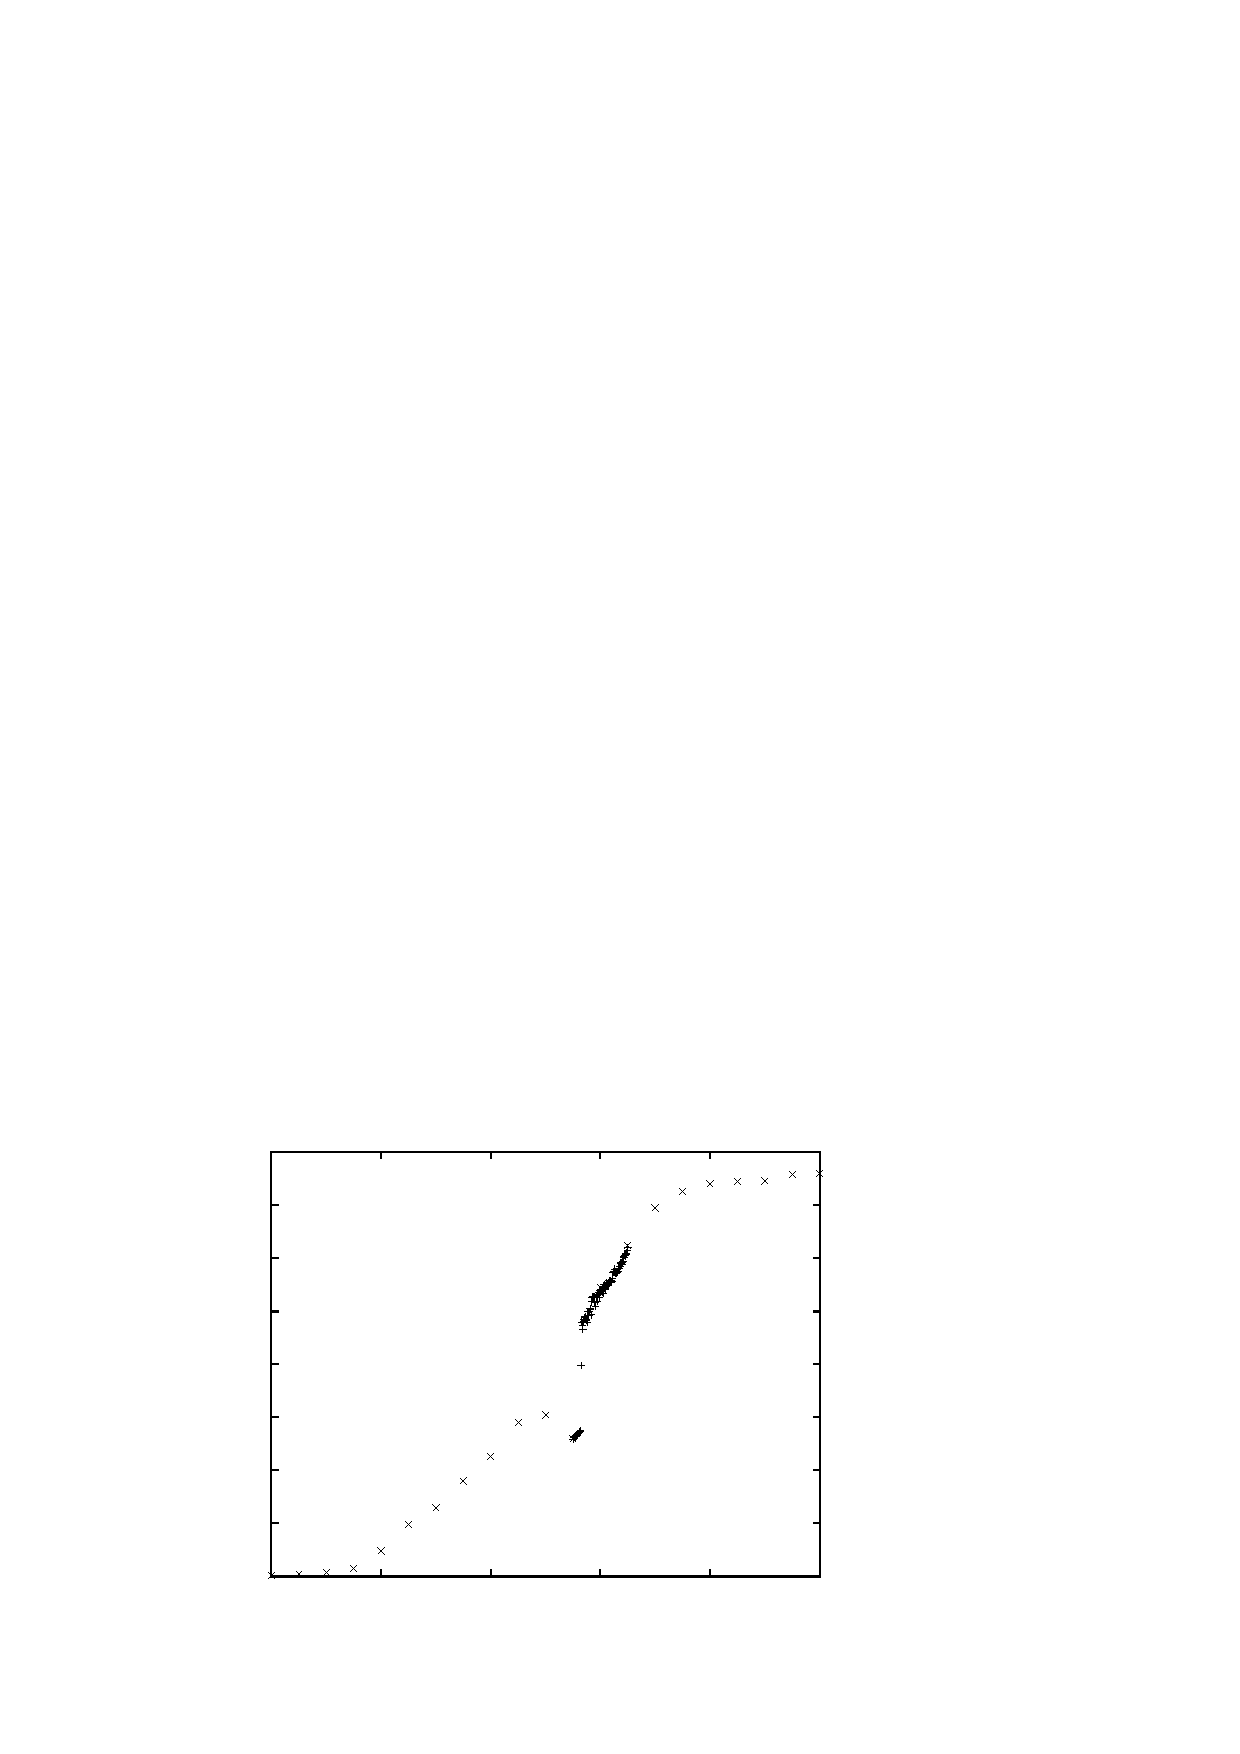
\includegraphics{2d1A}}%
    \gplfronttext
  \end{picture}%
\endgroup

\caption{Graf závislosti anodového proudu na napětí při magnetizačním proudu 2.1A.}
\end{figure}

\begin{figure}[h]
% GNUPLOT: LaTeX picture with Postscript
\begingroup
  \makeatletter
  \providecommand\color[2][]{%
    \GenericError{(gnuplot) \space\space\space\@spaces}{%
      Package color not loaded in conjunction with
      terminal option `colourtext'%
    }{See the gnuplot documentation for explanation.%
    }{Either use 'blacktext' in gnuplot or load the package
      color.sty in LaTeX.}%
    \renewcommand\color[2][]{}%
  }%
  \providecommand\includegraphics[2][]{%
    \GenericError{(gnuplot) \space\space\space\@spaces}{%
      Package graphicx or graphics not loaded%
    }{See the gnuplot documentation for explanation.%
    }{The gnuplot epslatex terminal needs graphicx.sty or graphics.sty.}%
    \renewcommand\includegraphics[2][]{}%
  }%
  \providecommand\rotatebox[2]{#2}%
  \@ifundefined{ifGPcolor}{%
    \newif\ifGPcolor
    \GPcolorfalse
  }{}%
  \@ifundefined{ifGPblacktext}{%
    \newif\ifGPblacktext
    \GPblacktexttrue
  }{}%
  % define a \g@addto@macro without @ in the name:
  \let\gplgaddtomacro\g@addto@macro
  % define empty templates for all commands taking text:
  \gdef\gplbacktext{}%
  \gdef\gplfronttext{}%
  \makeatother
  \ifGPblacktext
    % no textcolor at all
    \def\colorrgb#1{}%
    \def\colorgray#1{}%
  \else
    % gray or color?
    \ifGPcolor
      \def\colorrgb#1{\color[rgb]{#1}}%
      \def\colorgray#1{\color[gray]{#1}}%
      \expandafter\def\csname LTw\endcsname{\color{white}}%
      \expandafter\def\csname LTb\endcsname{\color{black}}%
      \expandafter\def\csname LTa\endcsname{\color{black}}%
      \expandafter\def\csname LT0\endcsname{\color[rgb]{1,0,0}}%
      \expandafter\def\csname LT1\endcsname{\color[rgb]{0,1,0}}%
      \expandafter\def\csname LT2\endcsname{\color[rgb]{0,0,1}}%
      \expandafter\def\csname LT3\endcsname{\color[rgb]{1,0,1}}%
      \expandafter\def\csname LT4\endcsname{\color[rgb]{0,1,1}}%
      \expandafter\def\csname LT5\endcsname{\color[rgb]{1,1,0}}%
      \expandafter\def\csname LT6\endcsname{\color[rgb]{0,0,0}}%
      \expandafter\def\csname LT7\endcsname{\color[rgb]{1,0.3,0}}%
      \expandafter\def\csname LT8\endcsname{\color[rgb]{0.5,0.5,0.5}}%
    \else
      % gray
      \def\colorrgb#1{\color{black}}%
      \def\colorgray#1{\color[gray]{#1}}%
      \expandafter\def\csname LTw\endcsname{\color{white}}%
      \expandafter\def\csname LTb\endcsname{\color{black}}%
      \expandafter\def\csname LTa\endcsname{\color{black}}%
      \expandafter\def\csname LT0\endcsname{\color{black}}%
      \expandafter\def\csname LT1\endcsname{\color{black}}%
      \expandafter\def\csname LT2\endcsname{\color{black}}%
      \expandafter\def\csname LT3\endcsname{\color{black}}%
      \expandafter\def\csname LT4\endcsname{\color{black}}%
      \expandafter\def\csname LT5\endcsname{\color{black}}%
      \expandafter\def\csname LT6\endcsname{\color{black}}%
      \expandafter\def\csname LT7\endcsname{\color{black}}%
      \expandafter\def\csname LT8\endcsname{\color{black}}%
    \fi
  \fi
  \setlength{\unitlength}{0.0500bp}%
  \begin{picture}(7200.00,5040.00)%
    \gplgaddtomacro\gplbacktext{%
      \csname LTb\endcsname%
      \put(1474,704){\makebox(0,0)[r]{\strut{} 0}}%
      \put(1474,1213){\makebox(0,0)[r]{\strut{} 0.0001}}%
      \put(1474,1722){\makebox(0,0)[r]{\strut{} 0.0002}}%
      \put(1474,2231){\makebox(0,0)[r]{\strut{} 0.0003}}%
      \put(1474,2740){\makebox(0,0)[r]{\strut{} 0.0004}}%
      \put(1474,3248){\makebox(0,0)[r]{\strut{} 0.0005}}%
      \put(1474,3757){\makebox(0,0)[r]{\strut{} 0.0006}}%
      \put(1474,4266){\makebox(0,0)[r]{\strut{} 0.0007}}%
      \put(1474,4775){\makebox(0,0)[r]{\strut{} 0.0008}}%
      \put(1606,484){\makebox(0,0){\strut{} 80}}%
      \put(2483,484){\makebox(0,0){\strut{} 100}}%
      \put(3360,484){\makebox(0,0){\strut{} 120}}%
      \put(4238,484){\makebox(0,0){\strut{} 140}}%
      \put(5115,484){\makebox(0,0){\strut{} 160}}%
      \put(5992,484){\makebox(0,0){\strut{} 180}}%
      \put(6869,484){\makebox(0,0){\strut{} 200}}%
      \put(308,2739){\rotatebox{-270}{\makebox(0,0){\strut{}$I_A$/A}}}%
      \put(4237,154){\makebox(0,0){\strut{}$U_A$/V}}%
    }%
    \gplgaddtomacro\gplfronttext{%
    }%
    \gplbacktext
    \put(0,0){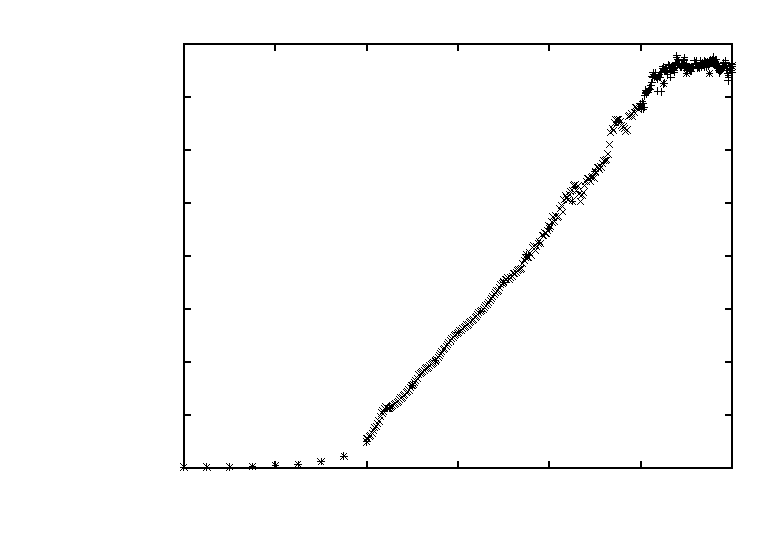
\includegraphics{2d3A}}%
    \gplfronttext
  \end{picture}%
\endgroup

\caption{Graf závislosti anodového proudu na napětí při magnetizačním proudu 2.3A.}
\end{figure}

\begin{figure}[h]
% GNUPLOT: LaTeX picture with Postscript
\begingroup
  \makeatletter
  \providecommand\color[2][]{%
    \GenericError{(gnuplot) \space\space\space\@spaces}{%
      Package color not loaded in conjunction with
      terminal option `colourtext'%
    }{See the gnuplot documentation for explanation.%
    }{Either use 'blacktext' in gnuplot or load the package
      color.sty in LaTeX.}%
    \renewcommand\color[2][]{}%
  }%
  \providecommand\includegraphics[2][]{%
    \GenericError{(gnuplot) \space\space\space\@spaces}{%
      Package graphicx or graphics not loaded%
    }{See the gnuplot documentation for explanation.%
    }{The gnuplot epslatex terminal needs graphicx.sty or graphics.sty.}%
    \renewcommand\includegraphics[2][]{}%
  }%
  \providecommand\rotatebox[2]{#2}%
  \@ifundefined{ifGPcolor}{%
    \newif\ifGPcolor
    \GPcolorfalse
  }{}%
  \@ifundefined{ifGPblacktext}{%
    \newif\ifGPblacktext
    \GPblacktexttrue
  }{}%
  % define a \g@addto@macro without @ in the name:
  \let\gplgaddtomacro\g@addto@macro
  % define empty templates for all commands taking text:
  \gdef\gplbacktext{}%
  \gdef\gplfronttext{}%
  \makeatother
  \ifGPblacktext
    % no textcolor at all
    \def\colorrgb#1{}%
    \def\colorgray#1{}%
  \else
    % gray or color?
    \ifGPcolor
      \def\colorrgb#1{\color[rgb]{#1}}%
      \def\colorgray#1{\color[gray]{#1}}%
      \expandafter\def\csname LTw\endcsname{\color{white}}%
      \expandafter\def\csname LTb\endcsname{\color{black}}%
      \expandafter\def\csname LTa\endcsname{\color{black}}%
      \expandafter\def\csname LT0\endcsname{\color[rgb]{1,0,0}}%
      \expandafter\def\csname LT1\endcsname{\color[rgb]{0,1,0}}%
      \expandafter\def\csname LT2\endcsname{\color[rgb]{0,0,1}}%
      \expandafter\def\csname LT3\endcsname{\color[rgb]{1,0,1}}%
      \expandafter\def\csname LT4\endcsname{\color[rgb]{0,1,1}}%
      \expandafter\def\csname LT5\endcsname{\color[rgb]{1,1,0}}%
      \expandafter\def\csname LT6\endcsname{\color[rgb]{0,0,0}}%
      \expandafter\def\csname LT7\endcsname{\color[rgb]{1,0.3,0}}%
      \expandafter\def\csname LT8\endcsname{\color[rgb]{0.5,0.5,0.5}}%
    \else
      % gray
      \def\colorrgb#1{\color{black}}%
      \def\colorgray#1{\color[gray]{#1}}%
      \expandafter\def\csname LTw\endcsname{\color{white}}%
      \expandafter\def\csname LTb\endcsname{\color{black}}%
      \expandafter\def\csname LTa\endcsname{\color{black}}%
      \expandafter\def\csname LT0\endcsname{\color{black}}%
      \expandafter\def\csname LT1\endcsname{\color{black}}%
      \expandafter\def\csname LT2\endcsname{\color{black}}%
      \expandafter\def\csname LT3\endcsname{\color{black}}%
      \expandafter\def\csname LT4\endcsname{\color{black}}%
      \expandafter\def\csname LT5\endcsname{\color{black}}%
      \expandafter\def\csname LT6\endcsname{\color{black}}%
      \expandafter\def\csname LT7\endcsname{\color{black}}%
      \expandafter\def\csname LT8\endcsname{\color{black}}%
    \fi
  \fi
  \setlength{\unitlength}{0.0500bp}%
  \begin{picture}(7200.00,5040.00)%
    \gplgaddtomacro\gplbacktext{%
      \csname LTb\endcsname%
      \put(1474,704){\makebox(0,0)[r]{\strut{} 0}}%
      \put(1474,1382){\makebox(0,0)[r]{\strut{} 0.0001}}%
      \put(1474,2061){\makebox(0,0)[r]{\strut{} 0.0002}}%
      \put(1474,2739){\makebox(0,0)[r]{\strut{} 0.0003}}%
      \put(1474,3418){\makebox(0,0)[r]{\strut{} 0.0004}}%
      \put(1474,4096){\makebox(0,0)[r]{\strut{} 0.0005}}%
      \put(1474,4775){\makebox(0,0)[r]{\strut{} 0.0006}}%
      \put(1606,484){\makebox(0,0){\strut{} 100}}%
      \put(2659,484){\makebox(0,0){\strut{} 120}}%
      \put(3711,484){\makebox(0,0){\strut{} 140}}%
      \put(4764,484){\makebox(0,0){\strut{} 160}}%
      \put(5816,484){\makebox(0,0){\strut{} 180}}%
      \put(6869,484){\makebox(0,0){\strut{} 200}}%
      \put(308,2739){\rotatebox{-270}{\makebox(0,0){\strut{}$I_A$/A}}}%
      \put(4237,154){\makebox(0,0){\strut{}$U_A$/V}}%
    }%
    \gplgaddtomacro\gplfronttext{%
    }%
    \gplbacktext
    \put(0,0){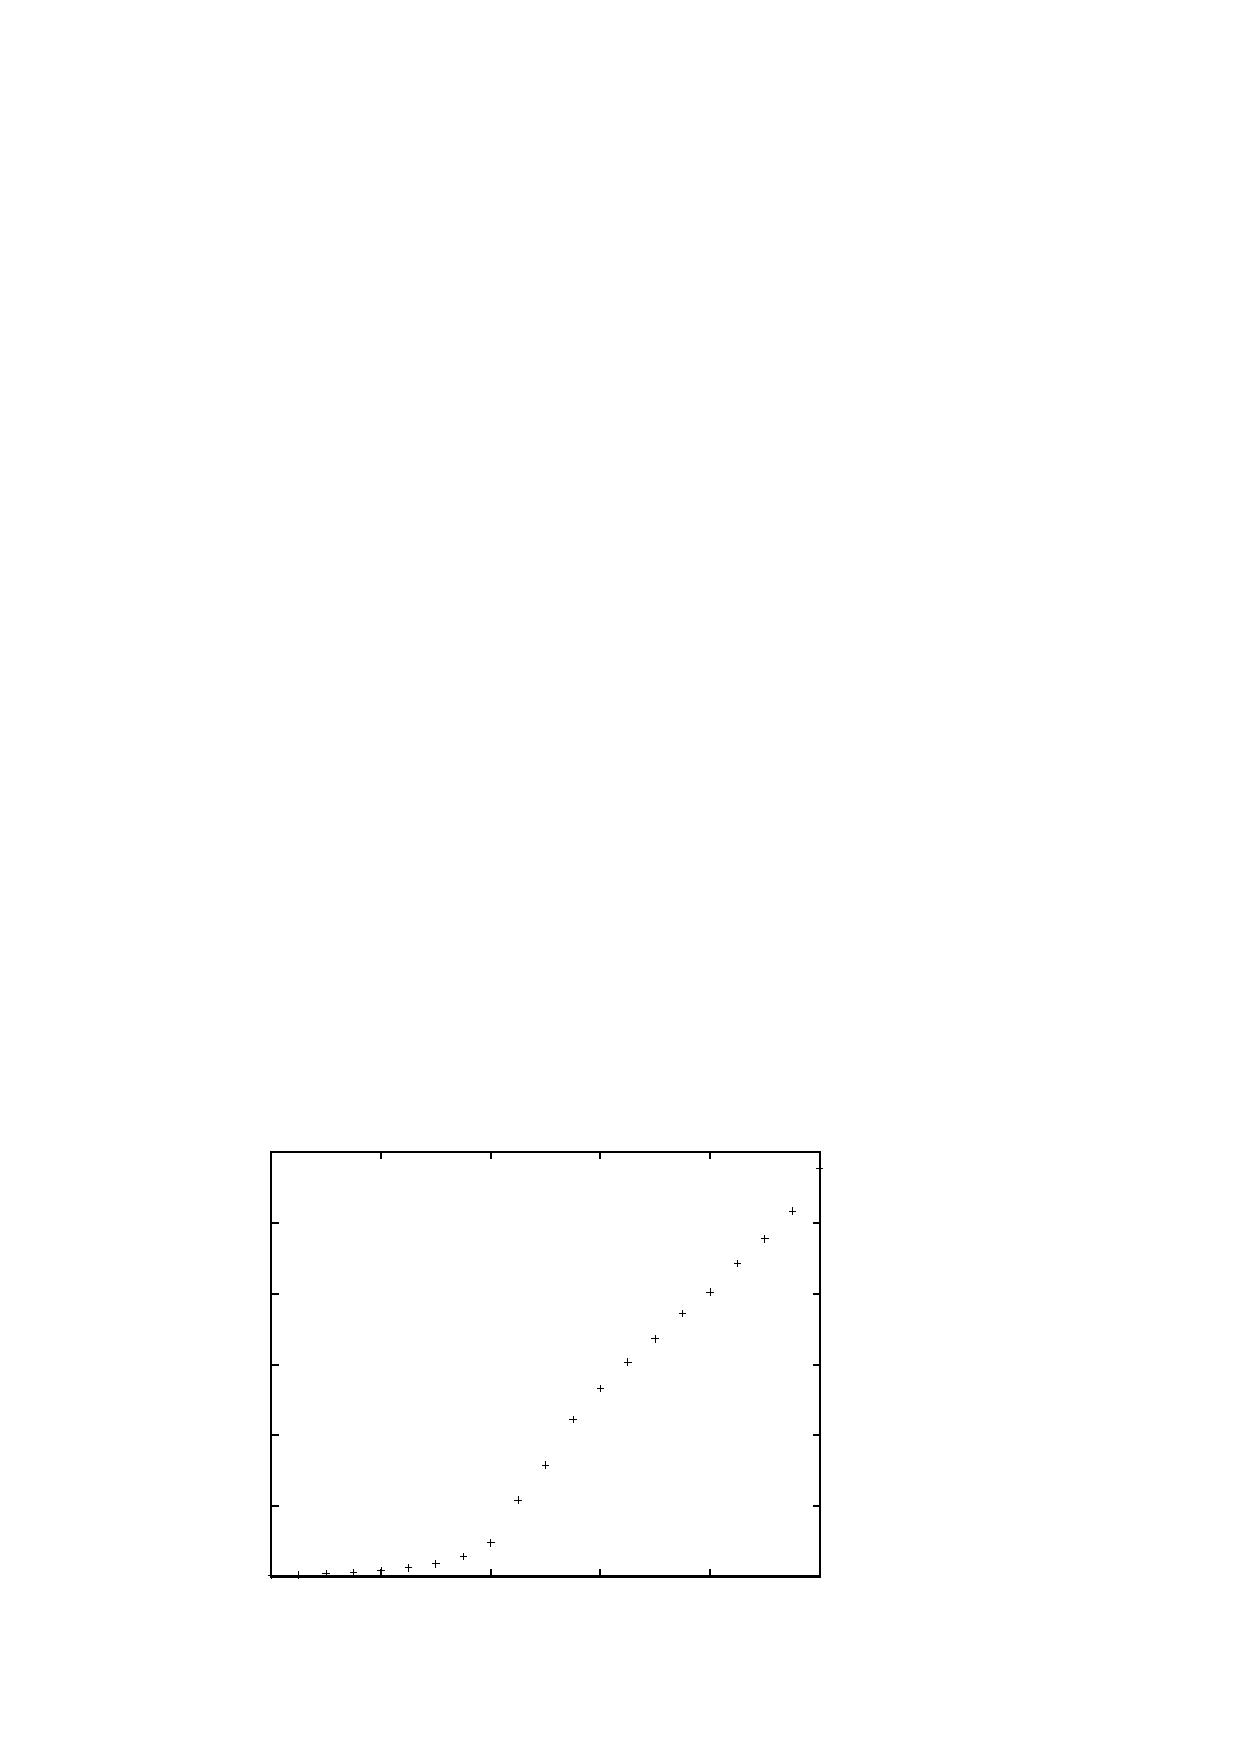
\includegraphics{2d5A}}%
    \gplfronttext
  \end{picture}%
\endgroup

\caption{Graf závislosti anodového proudu na napětí při magnetizačním proudu 2.5A.}
\label{posledni}
\end{figure}

\begin{figure}[h]
% GNUPLOT: LaTeX picture with Postscript
\begingroup
  \makeatletter
  \providecommand\color[2][]{%
    \GenericError{(gnuplot) \space\space\space\@spaces}{%
      Package color not loaded in conjunction with
      terminal option `colourtext'%
    }{See the gnuplot documentation for explanation.%
    }{Either use 'blacktext' in gnuplot or load the package
      color.sty in LaTeX.}%
    \renewcommand\color[2][]{}%
  }%
  \providecommand\includegraphics[2][]{%
    \GenericError{(gnuplot) \space\space\space\@spaces}{%
      Package graphicx or graphics not loaded%
    }{See the gnuplot documentation for explanation.%
    }{The gnuplot epslatex terminal needs graphicx.sty or graphics.sty.}%
    \renewcommand\includegraphics[2][]{}%
  }%
  \providecommand\rotatebox[2]{#2}%
  \@ifundefined{ifGPcolor}{%
    \newif\ifGPcolor
    \GPcolorfalse
  }{}%
  \@ifundefined{ifGPblacktext}{%
    \newif\ifGPblacktext
    \GPblacktexttrue
  }{}%
  % define a \g@addto@macro without @ in the name:
  \let\gplgaddtomacro\g@addto@macro
  % define empty templates for all commands taking text:
  \gdef\gplbacktext{}%
  \gdef\gplfronttext{}%
  \makeatother
  \ifGPblacktext
    % no textcolor at all
    \def\colorrgb#1{}%
    \def\colorgray#1{}%
  \else
    % gray or color?
    \ifGPcolor
      \def\colorrgb#1{\color[rgb]{#1}}%
      \def\colorgray#1{\color[gray]{#1}}%
      \expandafter\def\csname LTw\endcsname{\color{white}}%
      \expandafter\def\csname LTb\endcsname{\color{black}}%
      \expandafter\def\csname LTa\endcsname{\color{black}}%
      \expandafter\def\csname LT0\endcsname{\color[rgb]{1,0,0}}%
      \expandafter\def\csname LT1\endcsname{\color[rgb]{0,1,0}}%
      \expandafter\def\csname LT2\endcsname{\color[rgb]{0,0,1}}%
      \expandafter\def\csname LT3\endcsname{\color[rgb]{1,0,1}}%
      \expandafter\def\csname LT4\endcsname{\color[rgb]{0,1,1}}%
      \expandafter\def\csname LT5\endcsname{\color[rgb]{1,1,0}}%
      \expandafter\def\csname LT6\endcsname{\color[rgb]{0,0,0}}%
      \expandafter\def\csname LT7\endcsname{\color[rgb]{1,0.3,0}}%
      \expandafter\def\csname LT8\endcsname{\color[rgb]{0.5,0.5,0.5}}%
    \else
      % gray
      \def\colorrgb#1{\color{black}}%
      \def\colorgray#1{\color[gray]{#1}}%
      \expandafter\def\csname LTw\endcsname{\color{white}}%
      \expandafter\def\csname LTb\endcsname{\color{black}}%
      \expandafter\def\csname LTa\endcsname{\color{black}}%
      \expandafter\def\csname LT0\endcsname{\color{black}}%
      \expandafter\def\csname LT1\endcsname{\color{black}}%
      \expandafter\def\csname LT2\endcsname{\color{black}}%
      \expandafter\def\csname LT3\endcsname{\color{black}}%
      \expandafter\def\csname LT4\endcsname{\color{black}}%
      \expandafter\def\csname LT5\endcsname{\color{black}}%
      \expandafter\def\csname LT6\endcsname{\color{black}}%
      \expandafter\def\csname LT7\endcsname{\color{black}}%
      \expandafter\def\csname LT8\endcsname{\color{black}}%
    \fi
  \fi
  \setlength{\unitlength}{0.0500bp}%
  \begin{picture}(7200.00,5040.00)%
    \gplgaddtomacro\gplbacktext{%
      \csname LTb\endcsname%
      \put(1078,704){\makebox(0,0)[r]{\strut{} 0}}%
      \put(1078,1213){\makebox(0,0)[r]{\strut{} 20}}%
      \put(1078,1722){\makebox(0,0)[r]{\strut{} 40}}%
      \put(1078,2231){\makebox(0,0)[r]{\strut{} 60}}%
      \put(1078,2740){\makebox(0,0)[r]{\strut{} 80}}%
      \put(1078,3248){\makebox(0,0)[r]{\strut{} 100}}%
      \put(1078,3757){\makebox(0,0)[r]{\strut{} 120}}%
      \put(1078,4266){\makebox(0,0)[r]{\strut{} 140}}%
      \put(1078,4775){\makebox(0,0)[r]{\strut{} 160}}%
      \put(1210,484){\makebox(0,0){\strut{} 0.4}}%
      \put(1839,484){\makebox(0,0){\strut{} 0.6}}%
      \put(2468,484){\makebox(0,0){\strut{} 0.8}}%
      \put(3096,484){\makebox(0,0){\strut{} 1}}%
      \put(3725,484){\makebox(0,0){\strut{} 1.2}}%
      \put(4354,484){\makebox(0,0){\strut{} 1.4}}%
      \put(4983,484){\makebox(0,0){\strut{} 1.6}}%
      \put(5611,484){\makebox(0,0){\strut{} 1.8}}%
      \put(6240,484){\makebox(0,0){\strut{} 2}}%
      \put(6869,484){\makebox(0,0){\strut{} 2.2}}%
      \put(308,2739){\rotatebox{-270}{\makebox(0,0){\strut{}$U_k$/V}}}%
      \put(4039,154){\makebox(0,0){\strut{}$I_m$/A}}%
    }%
    \gplgaddtomacro\gplfronttext{%
    }%
    \gplbacktext
    \put(0,0){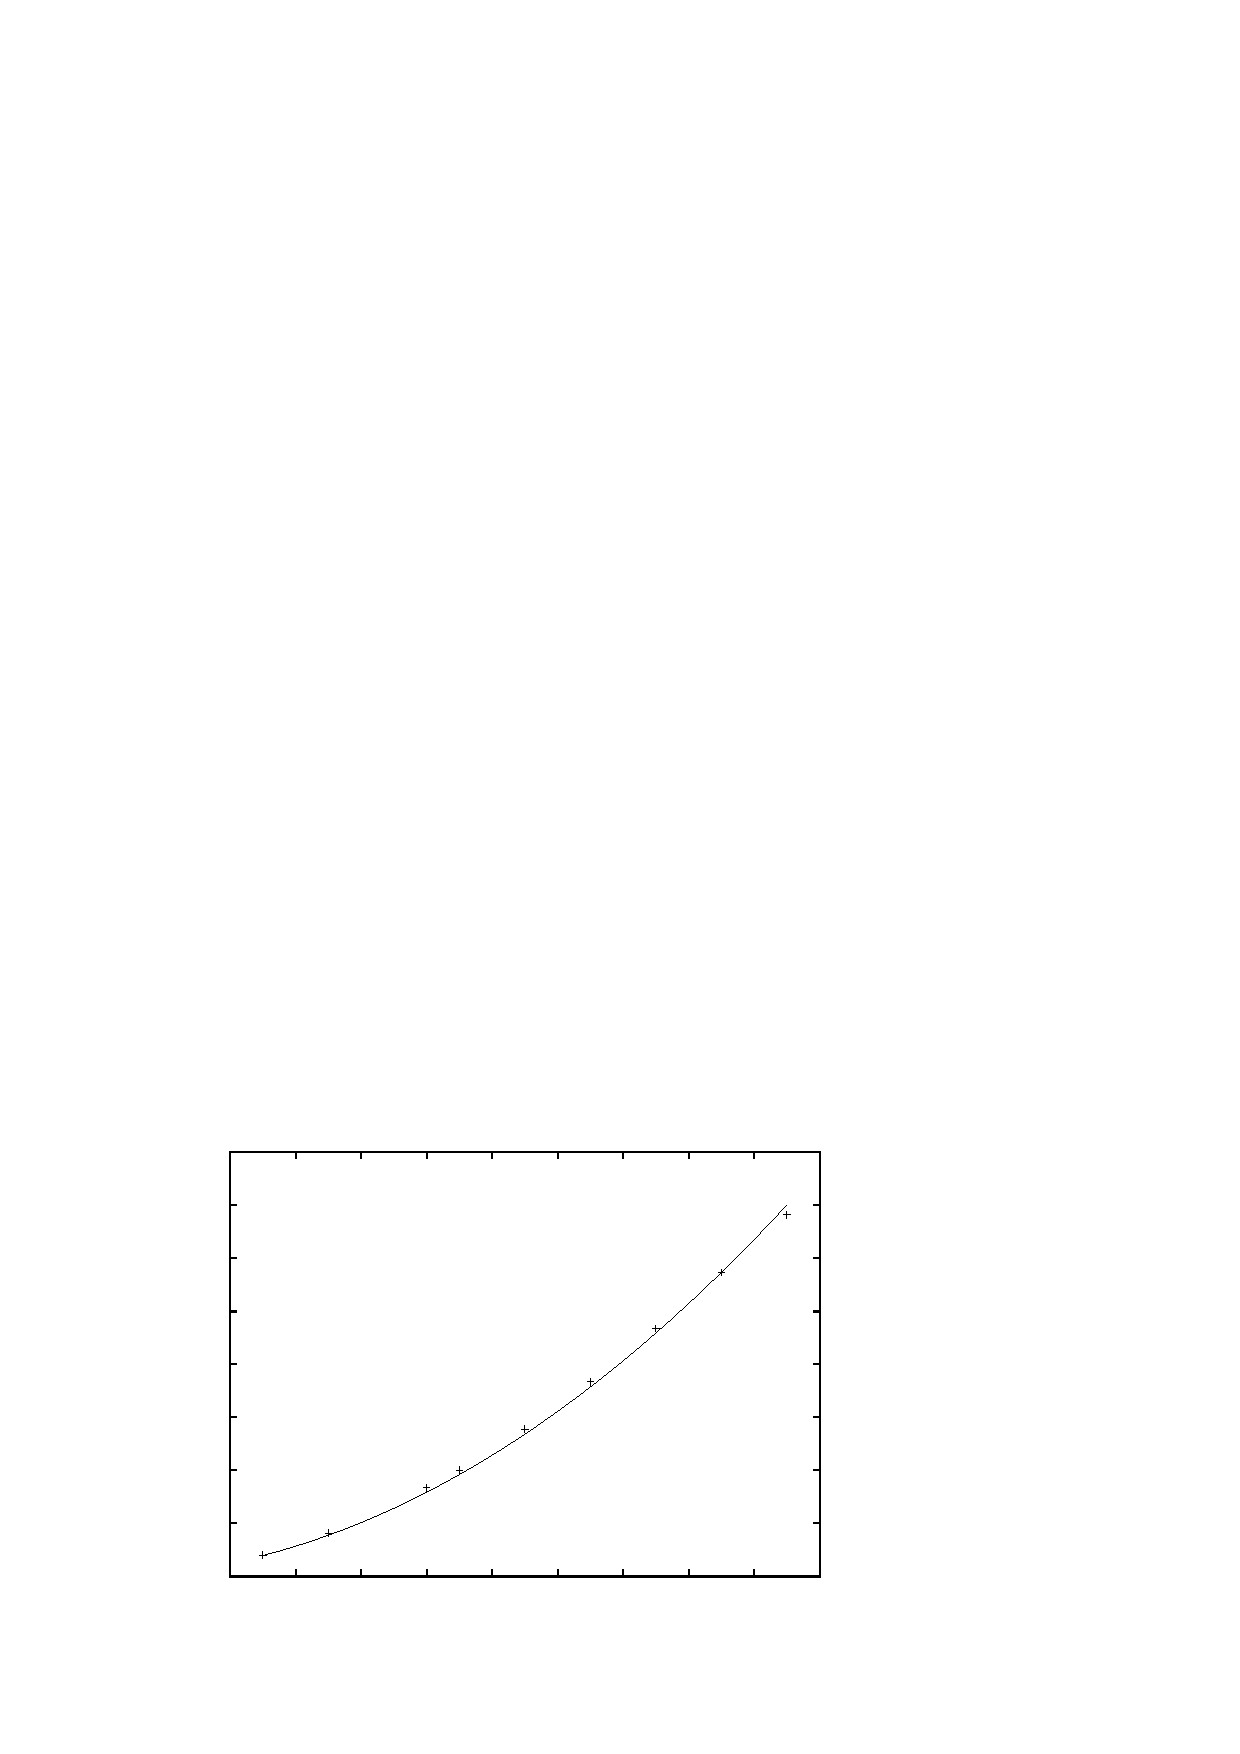
\includegraphics{Uk}}%
    \gplfronttext
  \end{picture}%
\endgroup

\caption{Graf závislosti kritického napětí na magnetozačním proudu s proloženou teoretickou závislostí.}
\label{GUk}
\end{figure}

\begin{figure}[h]
% GNUPLOT: LaTeX picture with Postscript
\begingroup
  \makeatletter
  \providecommand\color[2][]{%
    \GenericError{(gnuplot) \space\space\space\@spaces}{%
      Package color not loaded in conjunction with
      terminal option `colourtext'%
    }{See the gnuplot documentation for explanation.%
    }{Either use 'blacktext' in gnuplot or load the package
      color.sty in LaTeX.}%
    \renewcommand\color[2][]{}%
  }%
  \providecommand\includegraphics[2][]{%
    \GenericError{(gnuplot) \space\space\space\@spaces}{%
      Package graphicx or graphics not loaded%
    }{See the gnuplot documentation for explanation.%
    }{The gnuplot epslatex terminal needs graphicx.sty or graphics.sty.}%
    \renewcommand\includegraphics[2][]{}%
  }%
  \providecommand\rotatebox[2]{#2}%
  \@ifundefined{ifGPcolor}{%
    \newif\ifGPcolor
    \GPcolorfalse
  }{}%
  \@ifundefined{ifGPblacktext}{%
    \newif\ifGPblacktext
    \GPblacktexttrue
  }{}%
  % define a \g@addto@macro without @ in the name:
  \let\gplgaddtomacro\g@addto@macro
  % define empty templates for all commands taking text:
  \gdef\gplbacktext{}%
  \gdef\gplfronttext{}%
  \makeatother
  \ifGPblacktext
    % no textcolor at all
    \def\colorrgb#1{}%
    \def\colorgray#1{}%
  \else
    % gray or color?
    \ifGPcolor
      \def\colorrgb#1{\color[rgb]{#1}}%
      \def\colorgray#1{\color[gray]{#1}}%
      \expandafter\def\csname LTw\endcsname{\color{white}}%
      \expandafter\def\csname LTb\endcsname{\color{black}}%
      \expandafter\def\csname LTa\endcsname{\color{black}}%
      \expandafter\def\csname LT0\endcsname{\color[rgb]{1,0,0}}%
      \expandafter\def\csname LT1\endcsname{\color[rgb]{0,1,0}}%
      \expandafter\def\csname LT2\endcsname{\color[rgb]{0,0,1}}%
      \expandafter\def\csname LT3\endcsname{\color[rgb]{1,0,1}}%
      \expandafter\def\csname LT4\endcsname{\color[rgb]{0,1,1}}%
      \expandafter\def\csname LT5\endcsname{\color[rgb]{1,1,0}}%
      \expandafter\def\csname LT6\endcsname{\color[rgb]{0,0,0}}%
      \expandafter\def\csname LT7\endcsname{\color[rgb]{1,0.3,0}}%
      \expandafter\def\csname LT8\endcsname{\color[rgb]{0.5,0.5,0.5}}%
    \else
      % gray
      \def\colorrgb#1{\color{black}}%
      \def\colorgray#1{\color[gray]{#1}}%
      \expandafter\def\csname LTw\endcsname{\color{white}}%
      \expandafter\def\csname LTb\endcsname{\color{black}}%
      \expandafter\def\csname LTa\endcsname{\color{black}}%
      \expandafter\def\csname LT0\endcsname{\color{black}}%
      \expandafter\def\csname LT1\endcsname{\color{black}}%
      \expandafter\def\csname LT2\endcsname{\color{black}}%
      \expandafter\def\csname LT3\endcsname{\color{black}}%
      \expandafter\def\csname LT4\endcsname{\color{black}}%
      \expandafter\def\csname LT5\endcsname{\color{black}}%
      \expandafter\def\csname LT6\endcsname{\color{black}}%
      \expandafter\def\csname LT7\endcsname{\color{black}}%
      \expandafter\def\csname LT8\endcsname{\color{black}}%
    \fi
  \fi
  \setlength{\unitlength}{0.0500bp}%
  \begin{picture}(7200.00,5040.00)%
    \gplgaddtomacro\gplbacktext{%
      \csname LTb\endcsname%
      \put(814,704){\makebox(0,0)[r]{\strut{} 0}}%
      \put(814,1213){\makebox(0,0)[r]{\strut{} 1}}%
      \put(814,1722){\makebox(0,0)[r]{\strut{} 2}}%
      \put(814,2231){\makebox(0,0)[r]{\strut{} 3}}%
      \put(814,2740){\makebox(0,0)[r]{\strut{} 4}}%
      \put(814,3248){\makebox(0,0)[r]{\strut{} 5}}%
      \put(814,3757){\makebox(0,0)[r]{\strut{} 6}}%
      \put(814,4266){\makebox(0,0)[r]{\strut{} 7}}%
      \put(814,4775){\makebox(0,0)[r]{\strut{} 8}}%
      \put(946,484){\makebox(0,0){\strut{} 0}}%
      \put(2131,484){\makebox(0,0){\strut{} 0.5}}%
      \put(3315,484){\makebox(0,0){\strut{} 1}}%
      \put(4500,484){\makebox(0,0){\strut{} 1.5}}%
      \put(5684,484){\makebox(0,0){\strut{} 2}}%
      \put(6869,484){\makebox(0,0){\strut{} 2.5}}%
      \put(308,2739){\rotatebox{-270}{\makebox(0,0){\strut{}$I_Acdot 10^{-4}$/A}}}%
      \put(3907,154){\makebox(0,0){\strut{}$I_m$/A}}%
    }%
    \gplgaddtomacro\gplfronttext{%
      \csname LTb\endcsname%
      \put(1738,3077){\makebox(0,0)[r]{\strut{}0 V}}%
      \csname LTb\endcsname%
      \put(1738,2857){\makebox(0,0)[r]{\strut{}20 V}}%
      \csname LTb\endcsname%
      \put(1738,2637){\makebox(0,0)[r]{\strut{}40 V}}%
      \csname LTb\endcsname%
      \put(1738,2417){\makebox(0,0)[r]{\strut{}60 V}}%
      \csname LTb\endcsname%
      \put(1738,2197){\makebox(0,0)[r]{\strut{}80 V}}%
      \csname LTb\endcsname%
      \put(1738,1977){\makebox(0,0)[r]{\strut{}100 V}}%
      \csname LTb\endcsname%
      \put(1738,1757){\makebox(0,0)[r]{\strut{}120 V}}%
      \csname LTb\endcsname%
      \put(1738,1537){\makebox(0,0)[r]{\strut{}140 V}}%
      \csname LTb\endcsname%
      \put(1738,1317){\makebox(0,0)[r]{\strut{}160 V}}%
      \csname LTb\endcsname%
      \put(1738,1097){\makebox(0,0)[r]{\strut{}180 V}}%
      \csname LTb\endcsname%
      \put(1738,877){\makebox(0,0)[r]{\strut{}200 V}}%
    }%
    \gplbacktext
    \put(0,0){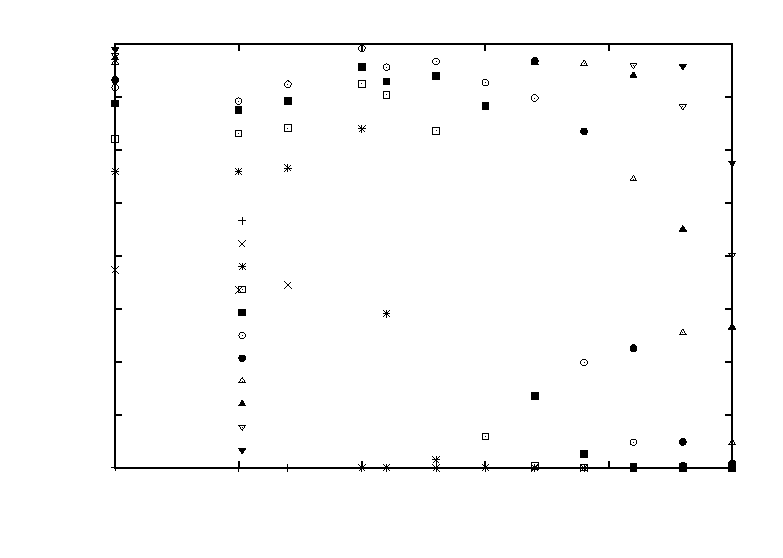
\includegraphics{UB}}%
    \gplfronttext
  \end{picture}%
\endgroup

\caption{Graf závislosti anodového proudu na magnetizačním proudu pro konstantní anodové napětí.}
\label{GUB}
\end{figure}

\section{Diskuze}
Jak je vidět na grafech, naměřené hodnoty odpovídají teoretickému předpokladu. Neočekávanou odchylkou je "kopec", který je těsně před kritickým napětím. Při nižším magnetizačním proudu byl nevýrazný, ale k závěru překryl 
toto napětí a proto nebylo možné ho určit.

Při určování měrného náboje došlo k velmi hrubé chybě. Když vyloučím chybu na mé straně, kterou se mi nepodařilo odhalit, zbývají jen dvě možné alternativy. Zaprvé parametry měřícího přístroje řádově nedpovádají údajům uvedeným 
v \cite{text}. Za druhé by nosiče náboje museli být velmo hmotné. Výsledek odpovídá iontům poměrně těžkých prvků, kterým sice Wolfram je, ale nemůžeme očekávat, že by bylo možné vythávat takovéto ionty z anody. Nejpravděpodobnější 
je tedy (po chybě ve zpravocání) jiná sada cívek použitá pro vytváření magnetického pole, případně použití jádra.

Z důvodu nejistoty při určení magnetické iindukce jsem poslední graf ze zadání raději vynesl v závislosti na magnetizačním proudu. To nemá na fyzikální význam grafu žádný vliv, protože se jedná pouze o přeškálování konstantou.

\eject

\section{Závěr}
Změřil jsem VA charakteristiku magnetronu pro různé magnetizační proudy. Výsledky jsou na obrázcích (\ref{prvni}) až (\ref{posledni}) \\
Určil jsem hodnoty kritických napětí, které jsou shrnuty v tabulce \ref{TUk}. \\
Nepodařilo se mi určit hondotu měrného náboje elektronu. \\
Setrojil jsem graf závislosti anodového proudu na proudu magnetizačním pro různá anodová napětí, který je na obrázku \ref{GUB}.


\begin{thebibliography}{5}
	\bibitem{text} \textbf{Studijní text na praktikum IV} \\http://physics.mff.cuni.cz/vyuka/zfp/txt\_414.pdf (21. 11. 2012)
\end{thebibliography}
\end{document}
